\documentclass[12pt]{article}
\usepackage[a4paper]{geometry}
\usepackage[myheadings]{fullpage}
\usepackage{fancyhdr}
\usepackage[table,xcdraw]{xcolor}
\usepackage{array,multirow,makecell}
\usepackage{lastpage}
\usepackage{graphicx, wrapfig, subcaption, setspace, booktabs}
\usepackage[T1]{fontenc}
\usepackage[font=small, labelfont=bf]{caption}
\usepackage{fourier}
\usepackage[protrusion=true, expansion=true]{microtype}
\usepackage[english]{babel}
\usepackage{sectsty}
\usepackage{url}
\usepackage{float}
\usepackage{fancyvrb}
\usepackage{enumerate}
\usepackage{enumitem}
\usepackage{mdframed}
\usepackage{soul}
\usepackage{amsmath}
\usepackage{amssymb}
\usepackage{alltt}
\usepackage{fullpage}
\usepackage[table,xcdraw]{xcolor}

\setcounter{tocdepth}{5}
\setcounter{secnumdepth}{5}

%-------------------------------------------------------------------------------
% HEADER & FOOTER
%-------------------------------------------------------------------------------
\pagestyle{fancy}
\fancyhf{}
\setlength\headheight{12pt}
\fancyhead[R]{Garza, Baker, and Sah \thepage}
\fancyhead[L]{Western Michigan University}
%-------------------------------------------------------------------------------
% TITLE PAGE
%-------------------------------------------------------------------------------
\begin{document}
\begin{titlepage}
  \newcommand{\HRule}{\rule{\linewidth}{0.5mm}} % Defines a new command for horizontal lines, change thickness here

  \center % Center everything on the page

  %----------------------------------------------------------------------------------------
  %	HEADER SECTION
  %----------------------------------------------------------------------------------------

  \textsc{\LARGE Western Michigan University}\\[0.5cm]
  \textsc{\Large Department of Electrical and Computer Engineering}\\[0.5cm] 
  \textsc{\large ECE-4820 Senior Design II}\\[0.5cm] 

  %----------------------------------------------------------------------------------------
  %	TITLE SECTION
  %----------------------------------------------------------------------------------------

  \HRule \\[0.4cm]
  { \huge \bfseries  Claims-Investigation Committee (CIC) Multi-Input Testing Device}\\[0.4cm]  
  \textsc{\Large Final Report }\\[0.4cm] 
  \HRule \\[1.5cm]

  %----------------------------------------------------------------------------------------
  %	LOGO SECTION
  %----------------------------------------------------------------------------------------

  
\includegraphics[width=0.3\textwidth]{./../assets/WMU_Logo.png}\\[1cm]  
  %----------------------------------------------------------------------------------------
  %	DATE SECTION
  %----------------------------------------------------------------------------------------

  {\large \today}\\[1cm] 

  %----------------------------------------------------------------------------------------
  %	ADVISOR & SPONSOR SECTION
  %----------------------------------------------------------------------------------------

  \begin{minipage}{0.4\textwidth}
    \begin{flushleft} \large
      \emph{Faculty Advisor:}\\
      Dr. Janos Grantner\\ [.25cm]
      \emph{Team Members:}\\
      Dylan-Matthew Garza\\
      Daniel Baker\\
      Rohullah Sah
    \end{flushleft}
  \end{minipage}
  ~
  \begin{minipage}{0.4\textwidth}
    \begin{flushright} \large
      \emph{Sponsor:} \\
      ZF
      \\\emph{Contact:}\\
      Patrick McNally\\ 
      Patrick.McNally@zf.com
    \end{flushright}
  \end{minipage}\\[1cm]

  %----------------------------------------------------------------------------------------
  %	TEAM MEMBERS SECTION
  %----------------------------------------------------------------------------------------

  \begin{flushleft} \large
  \end{flushleft}

  \vfill 

\end{titlepage}

\tableofcontents
\newpage
\
%----------------------------------------------------------------------------------------
%	PAPER BEGINS WITH ABSTRACT
%----------------------------------------------------------------------------------------
\section{Abstract}


This senior design project developed a comprehensive testing platform for ZF Group's 
automotive sensor validation, focusing on the Brake Signal Transmitter (BST) and 
related safety components. The system utilizes a dual-core STM32MP157F-DK2 
microcontroller, combining an ARM Cortex-M4 for real-time signal processing with 
an ARM Cortex-A7 running a custom embedded Linux distribution for test management 
and user interaction.

The platform features a WebAssembly-based frontend interfacing with a Rust web 
server, enabling intuitive test configuration and real-time result monitoring. 
OpenAMP facilitates inter-processor communication between the Cortex-A7 and M4 
cores, allowing seamless data transfer between the test execution and management 
layers. The system validates various automotive sensors against manufacturer 
specifications, providing automated test execution and detailed reporting 
capabilities through CSV export.

This solution significantly improves testing efficiency compared to existing methods, 
offering a scalable architecture that supports multiple device types including the 
BST, Continuous Wear Sensor, and Electronic Stability Control Module. Built with 
industry-standard technologies and professional engineering practices, the system 
demonstrates innovative integration of embedded systems, web technologies, and 
real-time processing for industrial testing applications.

%----------------------------------------------------------------------------------------
%	OVERVIEW STARTING WITH INTRODUCTION
%----------------------------------------------------------------------------------------
\section{Introduction}
The Claims Investigation Committee Multi-Testing Input Device automates validation 
testing for ZF Group's automotive safety sensors. Built on the STM32MP157F-DK2 
platform, it combines an ARM Cortex-M4 for real-time signal processing with a 
Cortex-A7 running custom embedded Linux for test management.

The system features a WebAssembly frontend with a Rust backend, using OpenAMP for 
inter-processor communication. It processes PWM signals, analog inputs, and CAN 
communications to validate devices against manufacturer specifications. While 
primarily focused on Brake Signal Transmitter (BST) testing, the platform supports 
additional devices including Continuous Wear Sensors and Electronic Stability 
Control Modules.

This automated solution improves testing efficiency and consistency while 
maintaining automotive industry standards. Test results are available through CSV 
export, enabling detailed analysis and documentation of validation procedures.

%----------------------------------------------------------------------------------------
%	DISCUSSION PORTION
%----------------------------------------------------------------------------------------
\section{Discussion}
%----------------------------------------------------------------------------------------
%	Overview of Project
%----------------------------------------------------------------------------------------
\subsection{Background}

ZF Group, a global Tier 1 automotive supplier specializing in advanced safety 
systems, identified a need to enhance their Claims Investigation Center's (CIC) 
testing capabilities. Based at their North American headquarters in Auburn Hills, 
MI, the CIC analyzes field failure parts and validates warranty claims for 
commercial vehicles.

Our project addresses this need by developing an automated testing platform that 
streamlines the validation process for returned components. The system focuses 
particularly on safety-critical parts like the Brake Signal Transmitter, 
supporting the CIC's mission of efficient warranty claim processing and product 
quality improvement.


\subsection{Need Statement}
ZF Group urgently requires a modernized testing platform to address critical
limitations in their current validation system. The existing mBSP tester is
incompatible with new components, cannot support prototype testing, and creates
significant delays in product validation. With Daimler's new platform
implementation and increasing production volumes, ZF needs a flexible, unified
testing solution that can efficiently validate multiple safety-critical
components while reducing testing time and costs. This system must support both
current and future product lines while maintaining rigorous testing standards
for warranty claim validation.

\subsection{High-Level System Design}

\begin{figure}[H]
  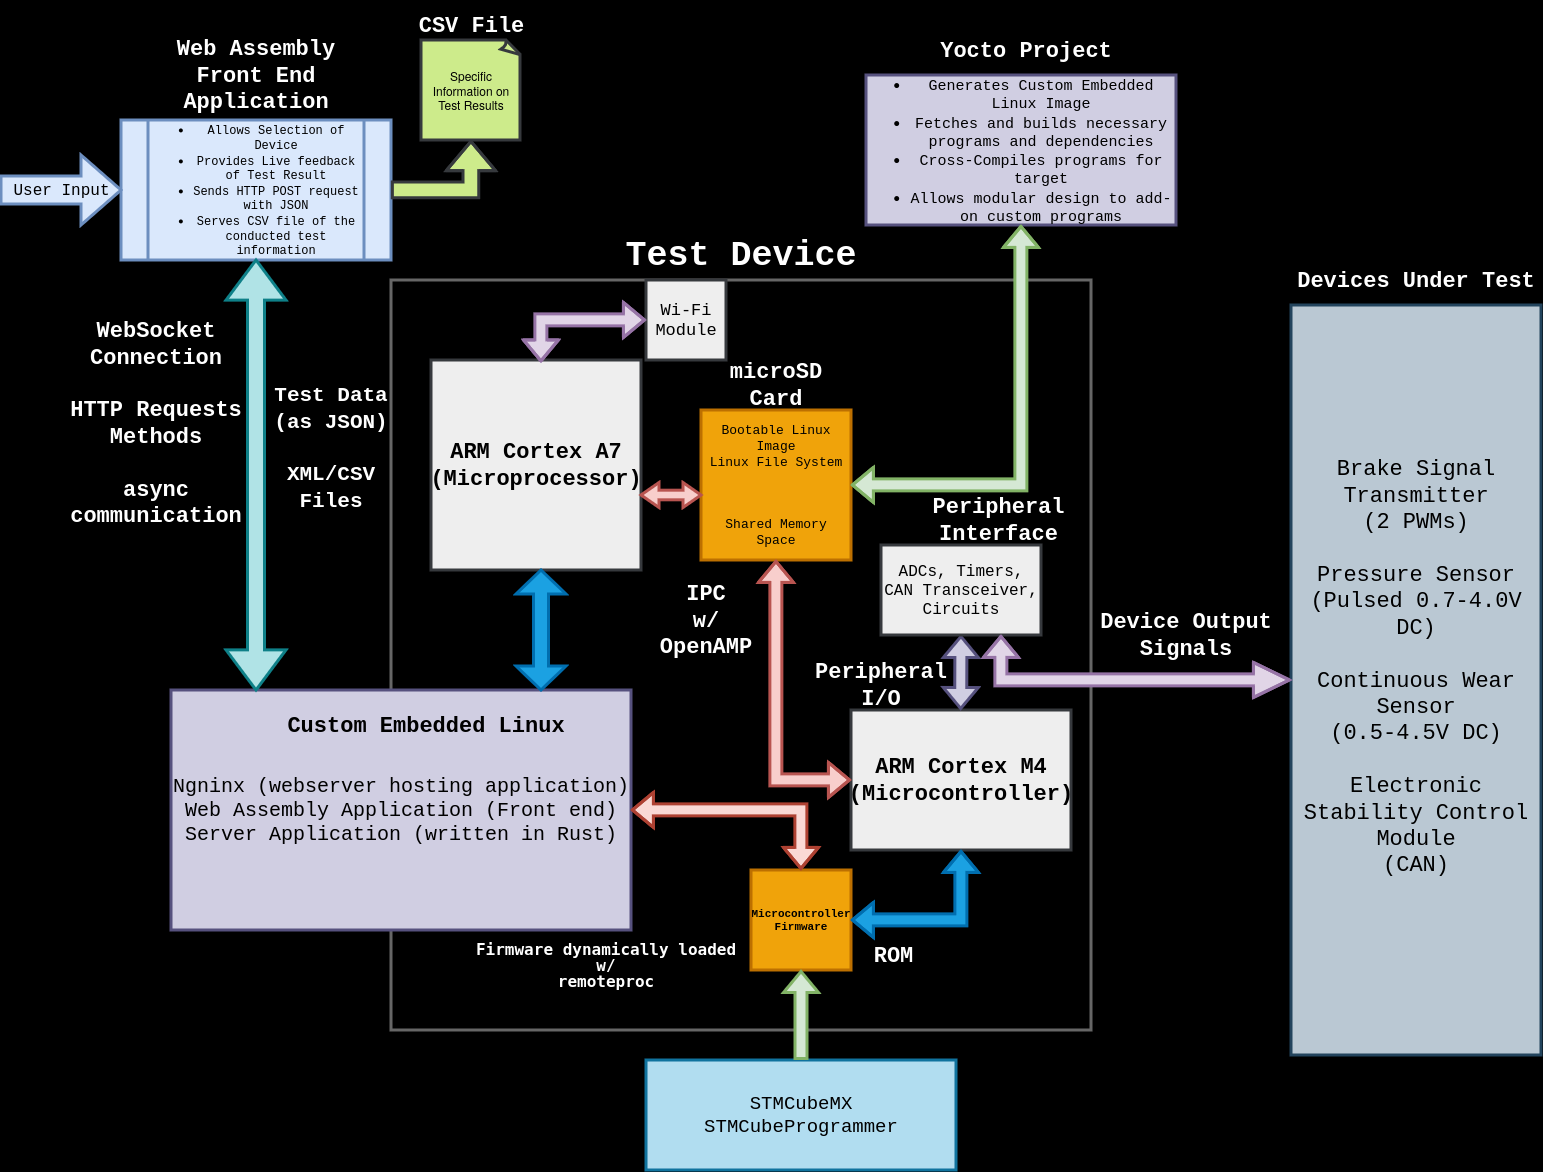
\includegraphics[width=\textwidth]{../assets/block_diagram.png}
  \caption{Comprehensive, High-level system block diagram}
\end{figure}

\subsection{Specifications}
\begin{enumerate}[label=\arabic*.]
  \item \textbf{Device Interfacing}
    \begin{enumerate}[label=\theenumi\arabic*]
      \item Properly read Device Signals using the ARM Cortex-M4 on the onboard 
        microcontroller on the STM32MP157F-DK2
        \begin{itemize}
          \item PWM duty cycle
          \item Frequency
          \item Voltages through an analog-to-digital converter (ADC)
          \item CAN frames
        \end{itemize}
    \end{enumerate}

  \item \textbf{Physical Components and Hardware}
    \begin{enumerate}[label=\theenumi\arabic*]
      \item Printed Circuit Board (PCB) for interfacing with DUT
      \item PCB for scaling and managing power for the DUT and to the 
        microcontroller
      \item Enclosure for PCBs and STM32MP157F-DK2 board
    \end{enumerate}

  \item \textbf{Software}
    \begin{enumerate}[label=\theenumi\arabic*]
      \item Custom embedded Linux distribution that will run on the onboard ARM 
        Cortex-A7 microprocessor on the STM32MP157F-DK2
      \item Simple user interface on web-based application
      \item Custom Webserver to process information from web application to 
        microcontroller
      \item Communicate collected information from ARM Cortex-M4 to ARM 
        Cortex-A7
      \item Ability to download measured data, formatted as a CSV, through the 
        web application
    \end{enumerate}
\end{enumerate}


\subsection{Deliverables}
The hardware component centers around custom circuit designs, featuring
\textbf{two specialized printed circuit boards}: a power management PCB that
handles voltage conversion and regulation, and a peripheral interface PCB that
manages signal routing and conditioning. Supporting these boards are
\textbf{protective enclosures} designed to house both the PCBs and the
STM32MP157F-DK2 development board, along with a comprehensive \textbf{wiring
harness system} for reliable device connections.

The software architecture comprises multiple integrated components. At its
foundation lies a \textbf{custom embedded Linux distribution} built using the
Yocto Project, which provides the operating system environment. User
interaction is handled through a \textbf{WebAssembly-based frontend interface}
that enables device selection and test control. A \textbf{Rust-based web
server} manages device communication and test execution. The system includes
specialized \textbf{ARM Cortex-M4 firmware} modules for testing various
devices: the Brake Signal Transmitter (BST) through PWM signal analysis, the
Continuous Wear Sensor (CWS) via voltage measurements, pressure sensor
validation, and Electronic Stability Control Module (ESCM) testing through CAN
communication.

The testing and documentation deliverables ensure system validation and future
maintainability. These include comprehensive \textbf{validation test results}
demonstrating compliance with manufacturer specifications, a \textbf{CSV data
export system} for maintaining test records, detailed \textbf{technical
documentation} covering system operation procedures, and organized
\textbf{source code repositories} with thorough documentation to support future
maintenance and upgrades. Together, these components form a unified testing
platform capable of handling multiple automotive sensor types while maintaining
strict compliance with ZF Group's testing requirements.

%----------------------------------------------------------------------------------------
%	Design and Implementation
% 
% * Hardware (Circuit/PCB) and device interfacing and power management
% * Enclosure Design
% * ARM Cortex-M4 Firmware
% * Embedded Linux with Yocto Project
% * Web Assembly application
% * Webserver
% * Inter-Processor Communication (IPC)
%----------------------------------------------------------------------------------------
\section{Design and Implementation}
\subsection{Devices Under Test (DUT)} The Claims Investigation Committee's
testing platform is designed to validate multiple critical automotive safety
components from ZF's commercial vehicle braking systems. These devices
represent key components in the braking system's safety chain, each serving
specific functions that together, ensure reliable and safe vehicle operation.

The testing platform currently supports four devices: the Brake Signal
Transmitter (BST), Continuous Wear Sensor (CWS), Electronic Stability Control
Module (ESCM), and a Pressure Sensor. Each device requires unique testing
approaches due to their distinct communication protocols and operational
parameters. Understanding these devices' functions and manufacturer
specifications is crucial for implementing accurate testing procedures. 

\subsubsection{Brake Signal Transmitter (BST)}

The Brake Signal Transmitter (BST) is a critical component in ZF's commercial
vehicle braking systems, providing real-time brake status information to the
vehicle's Electronic Control Unit (ECU). The Brake Signal Transmitter generates
the electrical and pneumatic signals that represent the braking demand of the
driver within the modular Braking System 2.0 (mBSP 2.0) Electronic Brake System
(EBS). The device has a single circuit pneumatic design and contains two
redundant pedal stroke sensors and a switch that is only used in European
design. To reduce the exhaust noise, the BST has a built-in silencer. The BST
is actuated by a foot pedal which is provided by the vehicle manufacturer (In
this case specifically Daimler Trucks North America). Two Pulse Width
Modulation (PWM) signals are generated by the BST, as long as both signals are
powered.

The BST's electrical architecture is designed for robust operation in
commercial vehicle environments. The BST uses a contact system of HDSCS by TYCO
(AMP MCP 1.5/2.8 MIX 7 - pole linear bayonet) for electrical connections.
Operating on a nominal 12V DC system, the device maintains functionality across
an 8V to 16V DC voltage range with built-in protection against reverse polarity
and overvoltage conditions. Each PWM channel draws no more than 50 mA current,
with total load capacitance limited to 6.8nF per channel. The output signals
are similarly protected, with maximum current limited to 15 mA per channel,
incorporating short-circuit protection and reverse polarity protection to
prevent damage to the device or the vehicle's electrical system.

The core functionality of the BST centers on its stroke sensor characteristics,
which generate two complementary PWM signals (S1 and S2) that precisely
indicate brake pedal position. These signals operate at 200Hz ±10Hz and follow
specific duty cycle relationships:

\begin{itemize} \item Signal S1 initiates at 12.5\% duty cycle when the brake
pedal is at rest (0mm stroke), increasing linearly at 5.96\% per millimeter of
pedal stroke. \item Signal S2 initiates at 87.5\% duty cycle when the brake
pedal is at rest (0mm stroke), decreasing linearly at 5.96\% per millimeter of
pedal stroke. \item Both signals maintain +- 5\% duty cycle tolerance
throughout the stroke range. \item The signals intersect at approximately 6.3mm
oedal stroke, with both signals at 50\% duty cycle. \end{itemize}

The PWM signals are defined by several key parameters: \begin{itemize} \item
Amplitude varying between U\textsubscript{max} (determined by CCU pull-up
voltage) and U\textsubscript{min} (<1V) \item Period T = 1/f, where f is the
200Hz carrier frequency \item Duty cycle calculated as DC =
T\textsubscript{high}/T\textsubscript{total} \end{itemize}

To ensure reliable signal integrity, the BST interface requires specific
loading conditions: \begin{itemize} \item Pull-up resistors: 4k$\Omega$
$\pm$1\% and 3k$\Omega$ $\pm$1\% to 12V \item Filtering capacitors: 2.2nF ±10\%
\end{itemize}

      The BST's implementation in Daimler's 2025 platform underscores the
      importance of accurate validation testing. As the highest volume
      commercial vehicle platform in North America, ensuring consistent and
      reliable BST operation is crucial for vehicle safety and warranty claim
      processing. This testing platform's ability to precisely measure PWM
      characteristics, timing relationships, and stroke correlations provides
      essential validation capabilities for both production quality assurance
      and field return analysis.


\subsubsection{Continuous Wear Sensor (CWS)} The Continuous Wear Sensor
represents a critical monitoring component in ZF's MAXX 2.0 air disc brake
generation for commercial vehicles, specifically designed for trucks and buses.
The sensor system integrates multiple functions to provide comprehensive brake
wear monitoring and maintenance capabilities.

The primary function of the CWS centers on precise wear measurement through
contactless sensing technology. Mounted directly on the disc brake caliper, the
sensor monitors the adjuster position to determine the collective wear state of
both brake pads and the brake disc rotor. This measurement is achieved through
a sophisticated distance-to-voltage conversion system that maintains both
linear and ratiometric characteristics, ensuring accurate wear detection
throughout the brake system's operational life.

A secondary but crucial feature of the CWS is its integrated re-adjustment
capability. A dedicated re-adjustment screw or shaft is incorporated into the
sensor design, enabling controlled retraction of the brake adjuster unit during
maintenance procedures. This integration streamlines service operations while
maintaining measurement accuracy.

The sensor's output signal serves multiple critical functions within the
Electronic Control Unit (ECU). These functions include continuous wear
monitoring, wear limit detection, predictive brake lining service forecasting,
wear harmonization across brake components, and comprehensive brake function
monitoring. This multi-faceted approach ensures both safety and maintenance
optimization.

The electrical architecture of the CWS is designed for robust operation in
commercial vehicle environments. The sensor utilizes a 3-pole BVA connector
system with specific pin assignments:

\begin{itemize} \item Supply Voltage (Us): 5V DC ±0.5V (Pin A) \item Output
Signal (Uout): 0.7V to 4.0V DC (Pin B) \item Ground Reference (Pin C)
\end{itemize}

The sensor's output characteristics follow a precise voltage-to-wear
relationship across four distinct operational ranges:

\begin{enumerate} \item New Brake Pad Condition \begin{itemize} \item Output
Voltage: 0.7V ±2\% (0.630V to 0.770V) \item Corresponding Position: 18.5mm
\end{itemize} \item Normal Wear Progression \begin{itemize} \item Output Range:
0.7V to 3.5V \item Position Range: 18.5mm to 53.5mm \item Linear voltage
increase with wear progression \end{itemize} \item Wear Limit Threshold
\begin{itemize} \item Output Voltage: 3.5V ±1\% (3.465V to 3.535V) \item
Corresponding Position: 53.5mm ±0.5mm \end{itemize} \item Worn Out Condition
\begin{itemize} \item Output Voltage: 4.0V ±5\% (3.8V to 4.2V) \item Position:
>53.5mm \end{itemize} \end{enumerate}

The electrical design incorporates multiple protection features to ensure
reliable operation. These include reverse polarity protection up to -5.5V DC,
short-circuit protection on the output signal, and current consumption limited
to 25mA maximum. When integrated with the ECU, the supply voltage is typically
pulsed rather than constant, optimizing power consumption while maintaining
measurement accuracy.

The CWS's ratiometric output characteristic ensures measurement stability
despite supply voltage fluctuations, as the output signal maintains its
proportional relationship to the input voltage. This design feature, combined
with the linear response to wear progression, enables precise wear monitoring
throughout the brake system's service life. The sensor's output is processed by
the ECU to provide real-time wear status information, enabling proactive
maintenance scheduling and ensuring optimal brake system performance.


\subsubsection{Electronic Stability Control Module (ESCM)}

\subsubsection{Pressure Sensor}

The pressure sensor represents a critical measurement component in ZF's
commercial vehicle control systems, serving as an actual-value transmitter for
continuous pressure monitoring. The sensor system integrates sophisticated
measurement technology with comprehensive protection features to ensure
reliable operation in demanding automotive environments.

The primary function of the pressure sensor centers on precise pressure
measurement through piezo-resistive sensing technology. A silicon diaphragm
forms the core sensing element, with measuring resistors precisely positioned
to form a Wheatstone bridge circuit. When pressure acts upon the diaphragm, the
resulting mechanical deformation induces proportional changes in the resistors'
values, creating a measurable electrical signal that accurately represents the
applied pressure relative to atmospheric conditions.

The sensor's signal processing capabilities represent a crucial aspect of its
design. The bridge output signal undergoes internal amplification and
calibration processes, with integrated temperature compensation ensuring
measurement stability. This sophisticated processing approach enables accurate
pressure monitoring across varying environmental conditions while maintaining
signal integrity throughout the measurement range.

The sensor's functionality extends beyond basic pressure measurement through
comprehensive protection features. The design incorporates reverse polarity
protection, overvoltage protection, and safeguards against high-frequency
disturbances. Combined with short-circuit protection, these features ensure
reliable operation in electro-pneumatic control systems where electrical noise
and power fluctuations are common challenges.

The electrical architecture of the pressure sensor is designed for robust
operation in commercial vehicle environments. The sensor utilizes a
standardized three-pole connector system with specific pin assignments:

\begin{itemize} \item Supply Voltage (UB): 8V to 32V DC (Pin 1) \item Output
Signal (Uout): 0.5V to 4.5V DC (Pin 2) \item Ground Reference (Pin 3)
\end{itemize}

The sensor's output characteristics follow a precise voltage-to-pressure
relationship with clearly defined parameters:

\begin{itemize} \item Offset voltage: 0.5V at atmospheric pressure (0 bar)
\item Linear sensitivity: 0.4V per bar across measurement range \item Maximum
output: 4.5V at full scale \item Characteristic limit: 4.7V ±100mV
\end{itemize}

The electrical design incorporates specific requirements for signal integrity
and protection. The output circuit requires minimum load impedances of 5.1k$\Omega$
to
ground and 68k$\Omega$ to supply voltage, ensuring reliable signal transmission.
Current consumption is limited to 15mA maximum, while operational readiness is
achieved within 10 milliseconds of power application, enabling rapid pressure
monitoring in dynamic vehicle systems.

The pressure sensor's ratiometric output characteristic ensures measurement
stability despite supply voltage fluctuations. This design feature, combined
with the sensor's broad operating voltage range and comprehensive protection
features, enables reliable pressure measurement in demanding automotive
applications. The sensor's output provides critical pressure information to the
vehicle's control systems, supporting safe and efficient operation of pneumatic
and hydraulic systems in commercial vehicles.

\subsection{Custom Printed Circuit Board for Device Interfacing and Power Management}
This project involved the development of schematic designs and custom PCBs to
manage power supply and interface with various devices under test (DUTs) using
KiCad. The designs were implemented to ensure stable power distribution and
accurate signal processing for the DUTs, with specific focus on hardware
efficiency and durability.


\subsubsection{Power Supply Schematic Design}
The power supply schematic begins with a 16V DC input, connected via a power
jack, which acts as the main source of power for the system. 10uF and 22uF
Capacitors are placed before and after each voltage regulator to ensure a
stable voltage level and filter out any electrical noise. These capacitors also
prevent voltage fluctuations, ensuring a stable supply to the components.
\break
\subsubsection*{Voltage Regulation}
  \begin{figure}[H]
    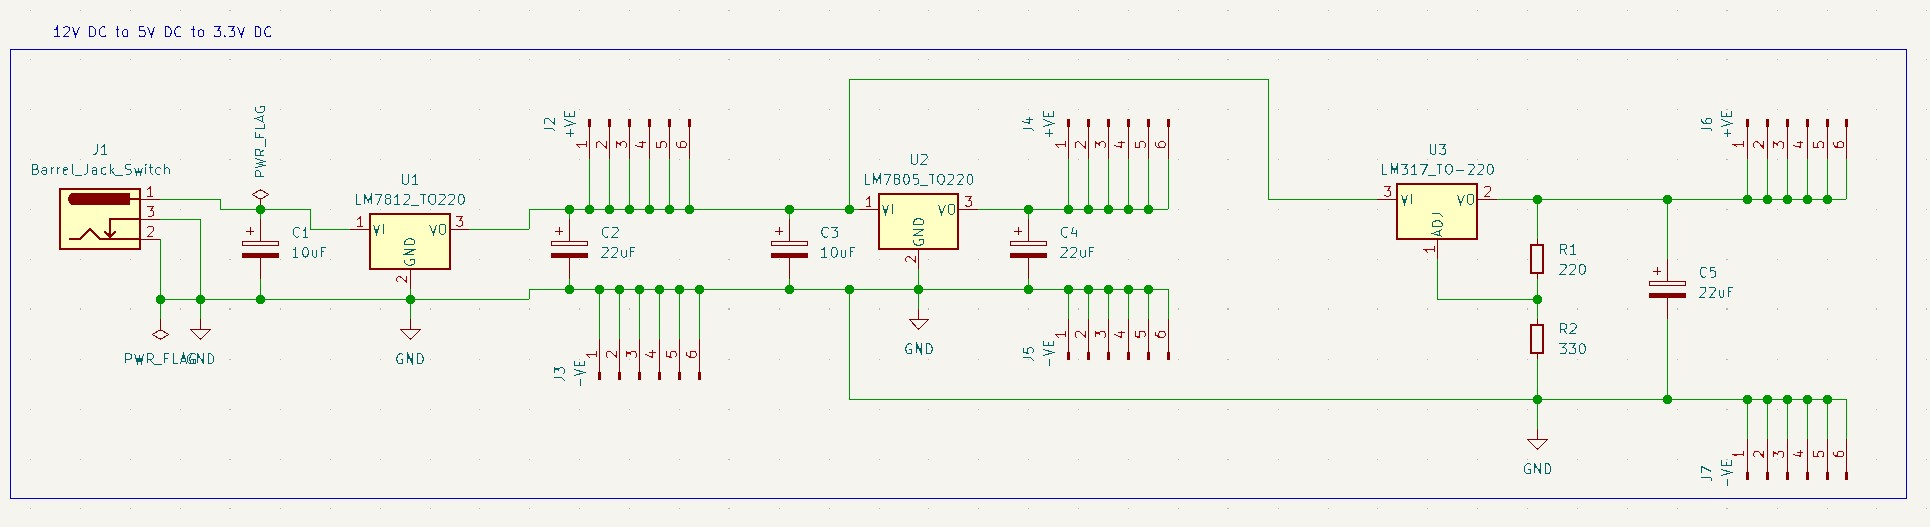
\includegraphics[width=\textwidth]{../assets/pcb/image1.jpg}
    \caption{Schematic Design of the Power Supply Management System}
  \end{figure}
\begin{itemize}
  \item The LM7812 voltage regulator converts the 16V DC input to 12V DC.
  \item The LM7805 voltage regulator further regulates the 12V DC to a 5V DC,
    suitable for devices that require low voltage.
  \item The LM317 adjustable regulator is used to step down the voltage for the
    microcontroller, providing a stable 3.146V DC. This precise voltage is
    achieved by using a combination of 220-ohm and 330-ohm resistors, which set
    the voltage according to the parameters.

    This layered voltage regulation ensures that all peripherals and the
    microcontroller receive clean and safe power levels for proper operation.
\end{itemize}

\subsubsection{Peripherals Schematic Design}
The peripherals schematic shows the design and signal conditioning circuits for
four Devices Under Test (DUT’s): the Brake Signal Transmitter (BST), the
Continuous Wear Sensor (CWS), the Pressure Sensor, and the String
Potentiometer. These circuits ensure accurate data acquisition and
compatibility with the STM32 Board by conditioning, scaling and protecting the
signals.

\subsubsection*{Brake Signal Transmitter}
The Brake Signal Transmitter is designed to read the Pulse Width Modulation
(PWM) signals, which represent the brake’s operational state. The circuit
includes resistors, such as 3k-ohms and 8.2k-ohms, to scale the PWM signals
down to levels safe for the microcontroller. Additionally, a 2.2nF capacitor is
used to filter out high-frequency noise, ensuring a clean and stable signal.
1N4001 diodes are included for overvoltage protection, safeguarding the
microcontroller from potential voltage spikes.

\begin{figure}[H]
  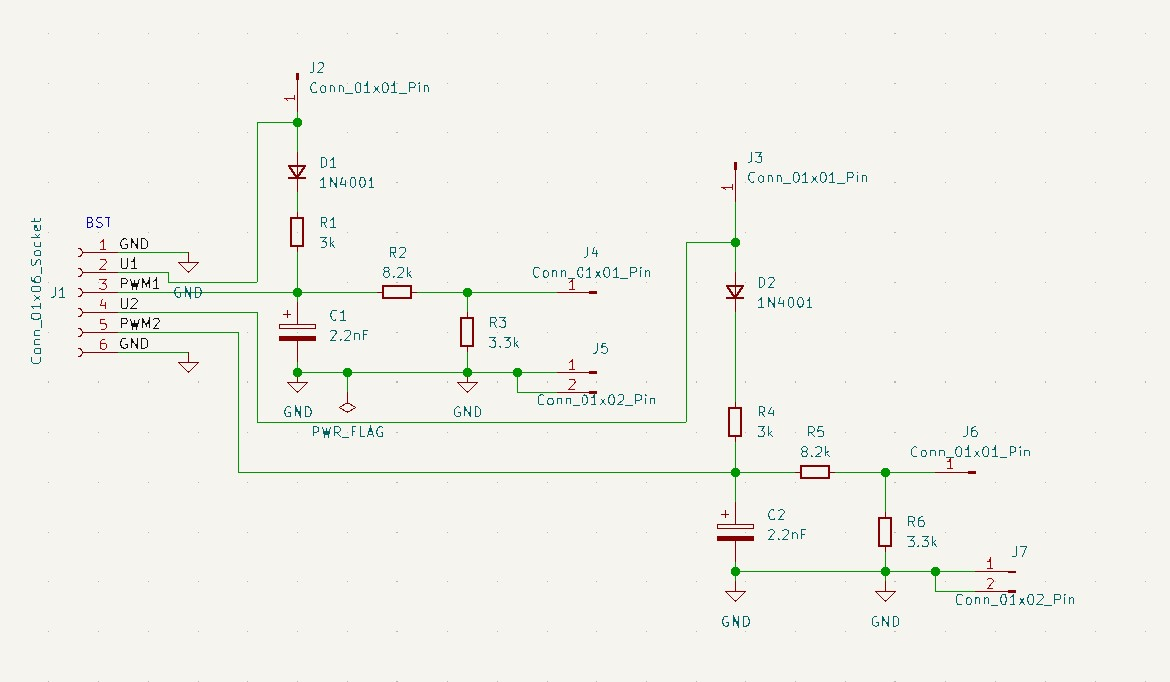
\includegraphics[width=\textwidth]{../assets/pcb/image2.jpg}
  \caption{Schematic Design of the Brake Signal Transmitter}
\end{figure}

\subsubsection*{Continuous Wear Sensor}
The Continuous Wear Sensor (CWS) captures analog voltage signals to monitor
brake pad wear. This schematic is relatively simple but effective, using
3k-ohms resistors for signal scaling and stabilization. Proper grounding
ensures that the integrity of the signal is minimized and maintain consistent
readings.

\begin{figure}[H]
  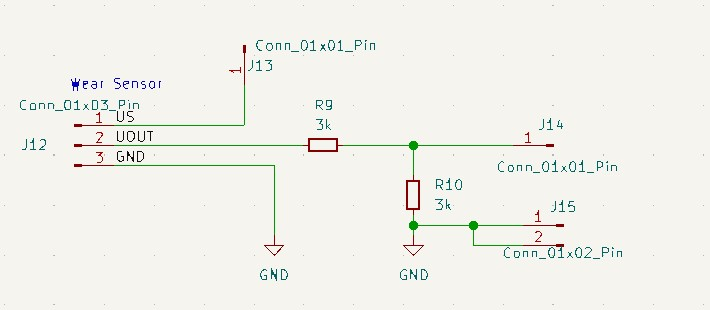
\includegraphics[width=\textwidth]{../assets/pcb/image3.jpg}
  \caption{Schematic Design of the Continuous Wear Sensor}
\end{figure}


\subsubsection*{Pressure Sensor}
The Pressure Sensor measures the pressure within the braking system. It outputs
an analog voltage signal, which is conditioned using a 330uF capacitor to
stabilize the output and eliminate fluctuations. Additionally, 3k-ohms
resistors are used to scale and prepare the signal for processing by the
microcontroller.

\begin{figure}[H]
  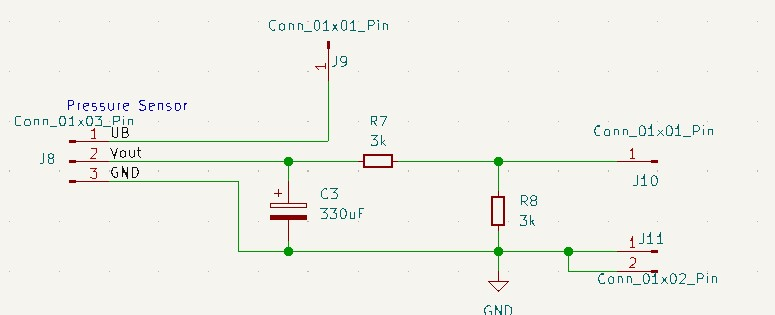
\includegraphics[width=\textwidth]{../assets/pcb/image4.jpg}
  \caption{Schematic Design of the Pressure Sensor}
\end{figure}

\subsubsection*{String Potentiometer}
The String Potentiometer is used to monitor the displacement, such as the
movement of the brake pedal, and converts it into proportional voltage signal.
This circuit uses resistors, including 8.5k-ohms and 3.3k-ohms, to scale the
output signal to levels suitable for the microcontroller. As with the other
peripherals, stable grounding and power inputs are implemented to maintain
accurate and reliable signal transmission.

\begin{figure}[H]
  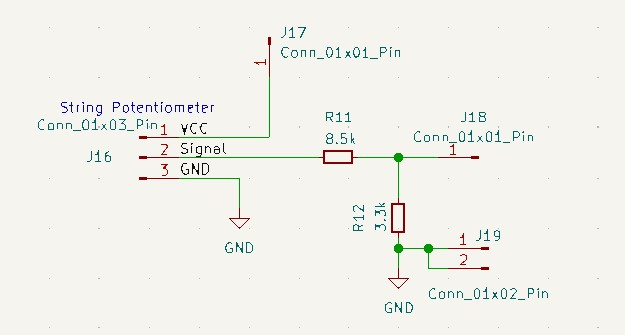
\includegraphics[width=\textwidth]{../assets/pcb/image5.jpg}
  \caption{Schematic Design of the String Potentiometer}
\end{figure}

Overall, the peripherals schematics focuses on providing clean, conditioned, and scaled signals from each DUT’s to the STM32 microcontroller while including corresponding components to prevent damage or errors. This ensures the entire system operates efficiently and reliably, with accurate data acquisition from all devices.

\subsubsection{Printed Circuit Board (PCB’s) Design}
\subsubsection*{Power Supply PCB}
The Power Supply PCB is a critical component designed to regulate and provide
multiple voltage levels to the system. It starts at 16V DC input through a
barrel jack connector. This 16V input is directed through a series of voltage
regulators that step down the voltage to meet the requirements of the various
components in the circuit.

The board utilizes capacitors of 10$\mu$F and 22$\mu$F, which are strategically placed
before and after each voltage regulator. These capacitors help to stabilize the
voltage output by filtering out noise and ensuring smooth operation. The LM7812
regulator steps down the voltage to 12V DC, which is essential for certain
peripherals. This 12V is then fed into another voltage regulator circuit
comprising an LM317 adjustable voltage regulator along with two resistors, 220$\Omega$
and 330$\Omega$, to further step it down to 3.146V DC. This precise voltage level is
crucial for the operation of the microcontroller.


The design includes multiple output pins for 12V, 5V, and 3.3V voltages,
ensuring compatibility with different devices and peripherals connected to the
system. The layout of the PCB is compact yet efficient, allowing for adequate
heat dissipation. The traces are kept wide enough to handle current flow
effectively, and proper spacing is maintained to prevent any electrical shorts.

\begin{figure}[H]
  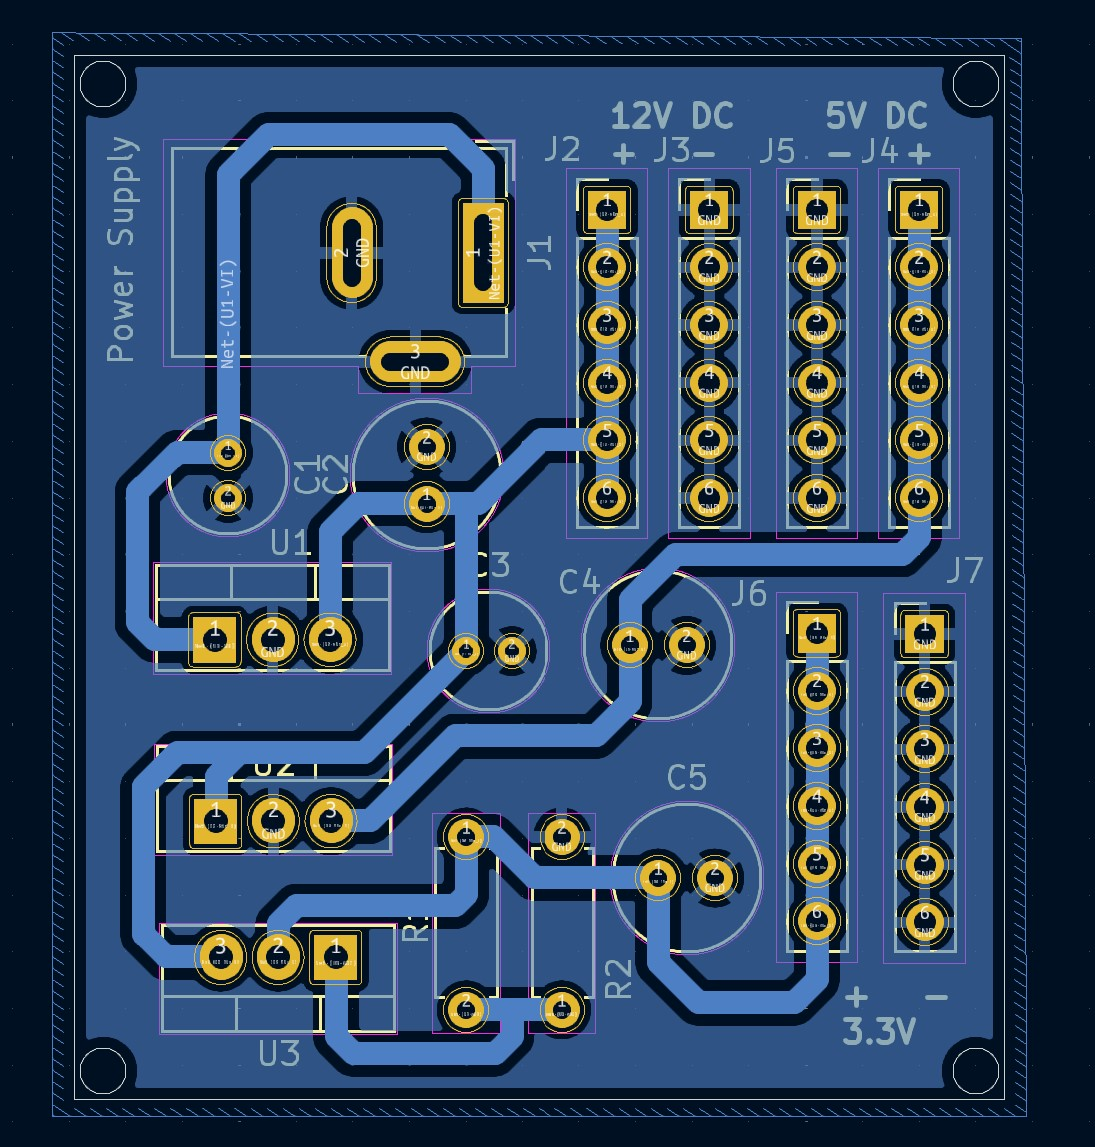
\includegraphics[width=\textwidth]{../assets/pcb/image6.jpg}
  \caption{Printed Circuit Board Design of the Power Supply Management}
\end{figure}
\subsubsection*{Peripheral PCB Design}
The Peripherals PCB is designed to accommodate all the connections and
conditioning circuits required for the various devices under test (DUTs),
including the Brake Signal Transmitter (BST), the Continuous Wear Sensor (CWS),
the Pressure Sensor, and the String Potentiometer. Each DUT is connected
through dedicated input and output pins, clearly labeled on the board for ease
of use.

The BST section includes diodes, resistors, and capacitors to read PWM signals
reliably. The diodes provide protection against voltage spikes, while the
resistors and capacitors condition the PWM signals for accurate processing.
Similarly, the Pressure Sensor section features a capacitor to stabilize the
signal and resistors to scale the output voltage for the microcontroller.

The Continuous Wear Sensor section captures analog voltage signals representing
brake wear. This signal is scaled and filtered using resistors and capacitors
to ensure accurate readings. The String Potentiometer section, on the other
hand, converts displacement into a proportional voltage signal. Resistors in
this section ensure the signal remains within the safe operating range for the
microcontroller.

The PCB layout emphasizes clean and efficient routing, ensuring that signals
are isolated to prevent interference. The components are arranged logically,
with each DUT section clearly mentioned, making the board easy to debug and
maintain.

Both the Power Supply and Peripherals PCBs were designed using KiCad, an
open-source PCB design tool. KiCad's features allowed precise component
placement and trace routing, ensuring reliable performance and
manufacturability of the boards. These PCBs were custom designed to meet the
specific requirements of the project, balancing functionality with simplicity.

\begin{figure}[H]
  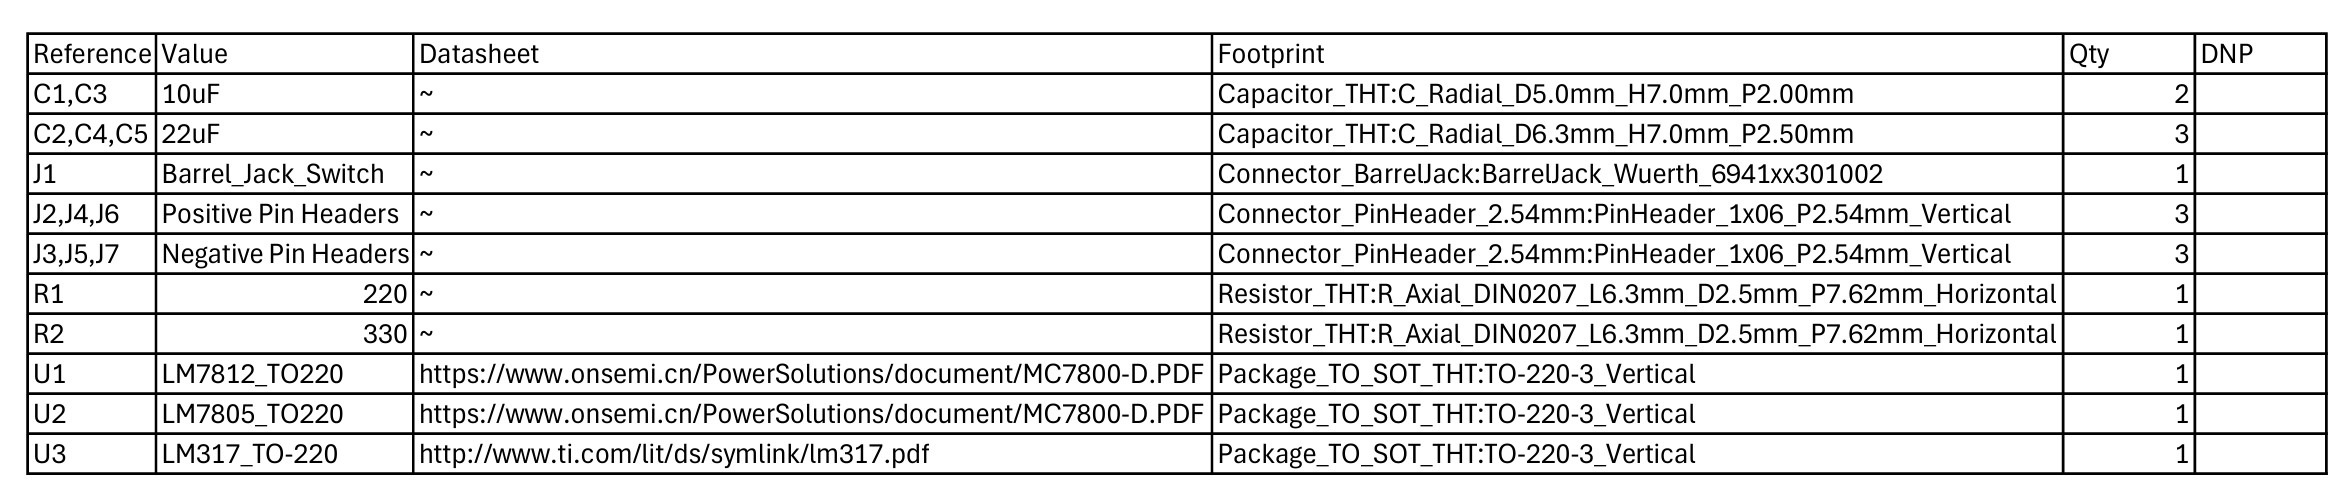
\includegraphics[width=\textwidth]{../assets/pcb/image7.jpg}
  \caption{Printed Circuit Board Design of the Peripherals}
\end{figure}
\subsubsection{Enclosure Design} 
The enclosures designed for the power supply
and peripherals PCBs, as well as the STM32 microcontroller, were custom-built
to meet the specific needs of the project. These enclosures were created using
Autodesk’s Fusion 360, allowing for precision in their design and ensuring they
provided both functional and inventive advantages.

\subsubsection*{Power Supply and Peripherals Enclosure} 
The combined enclosure
for the power supply and peripherals PCBs was designed with functionality as
the primary focus. It ensures the protection of the internal PCBs while also
providing easy access for connections and maintenance. Slots were strategically
placed for the DC jack and the input/output pins, which allowed efficient cable
management and straightforward connectivity during operation. Additionally,
ventilation slots were included to maintain stable temperatures and prevent
overheating during extended usage.

The interior design included standoffs to securely mount the PCBs, preventing
any physical movement that could damage connections. The two-part assembly of
the enclosure made it user-friendly for repairs, upgrades, or debugging tasks.
This modular design simplified the assembly and disassembly process while
ensuring durability.

\begin{figure}[H]
  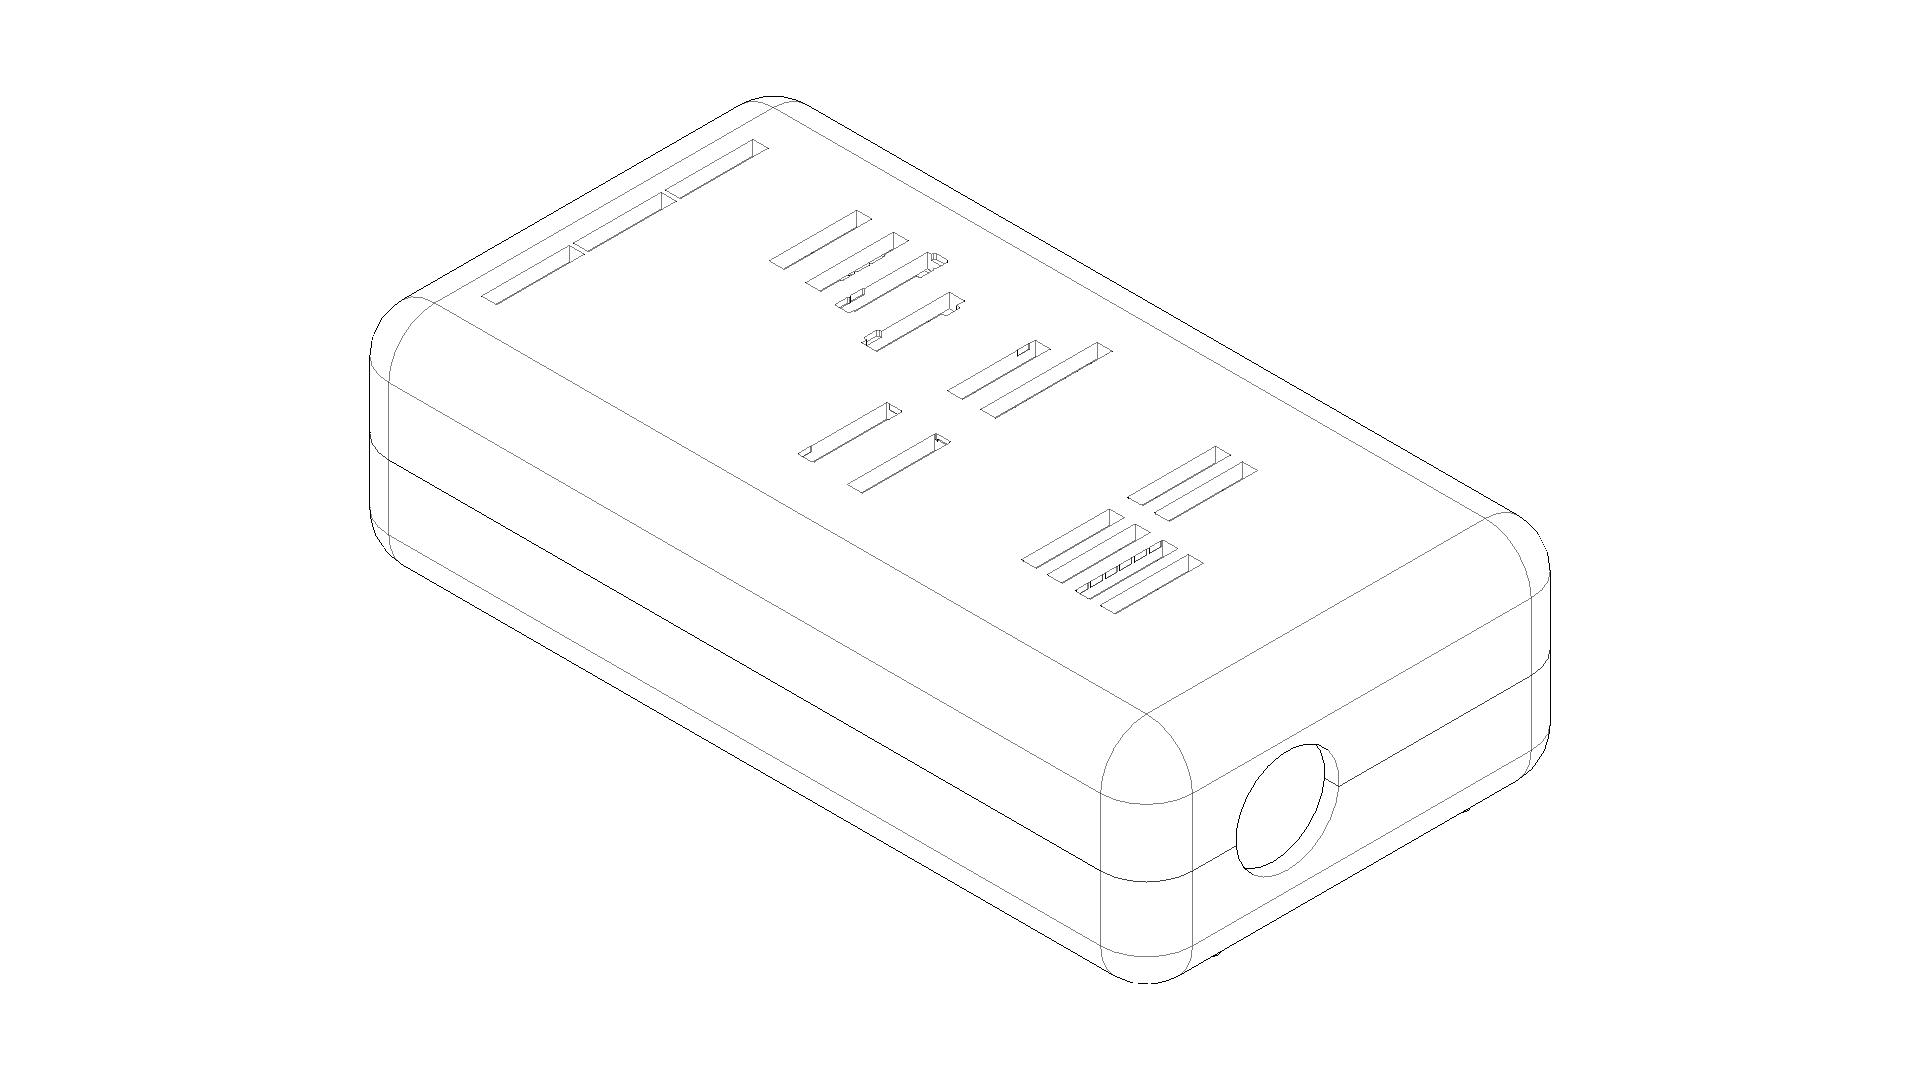
\includegraphics[width=\textwidth]{../assets/pcb/image8.jpg}
  \caption{Enclosed Enclosure for Power Supply PCB and Peripherals PCB}
\end{figure}

\begin{figure}[H]
  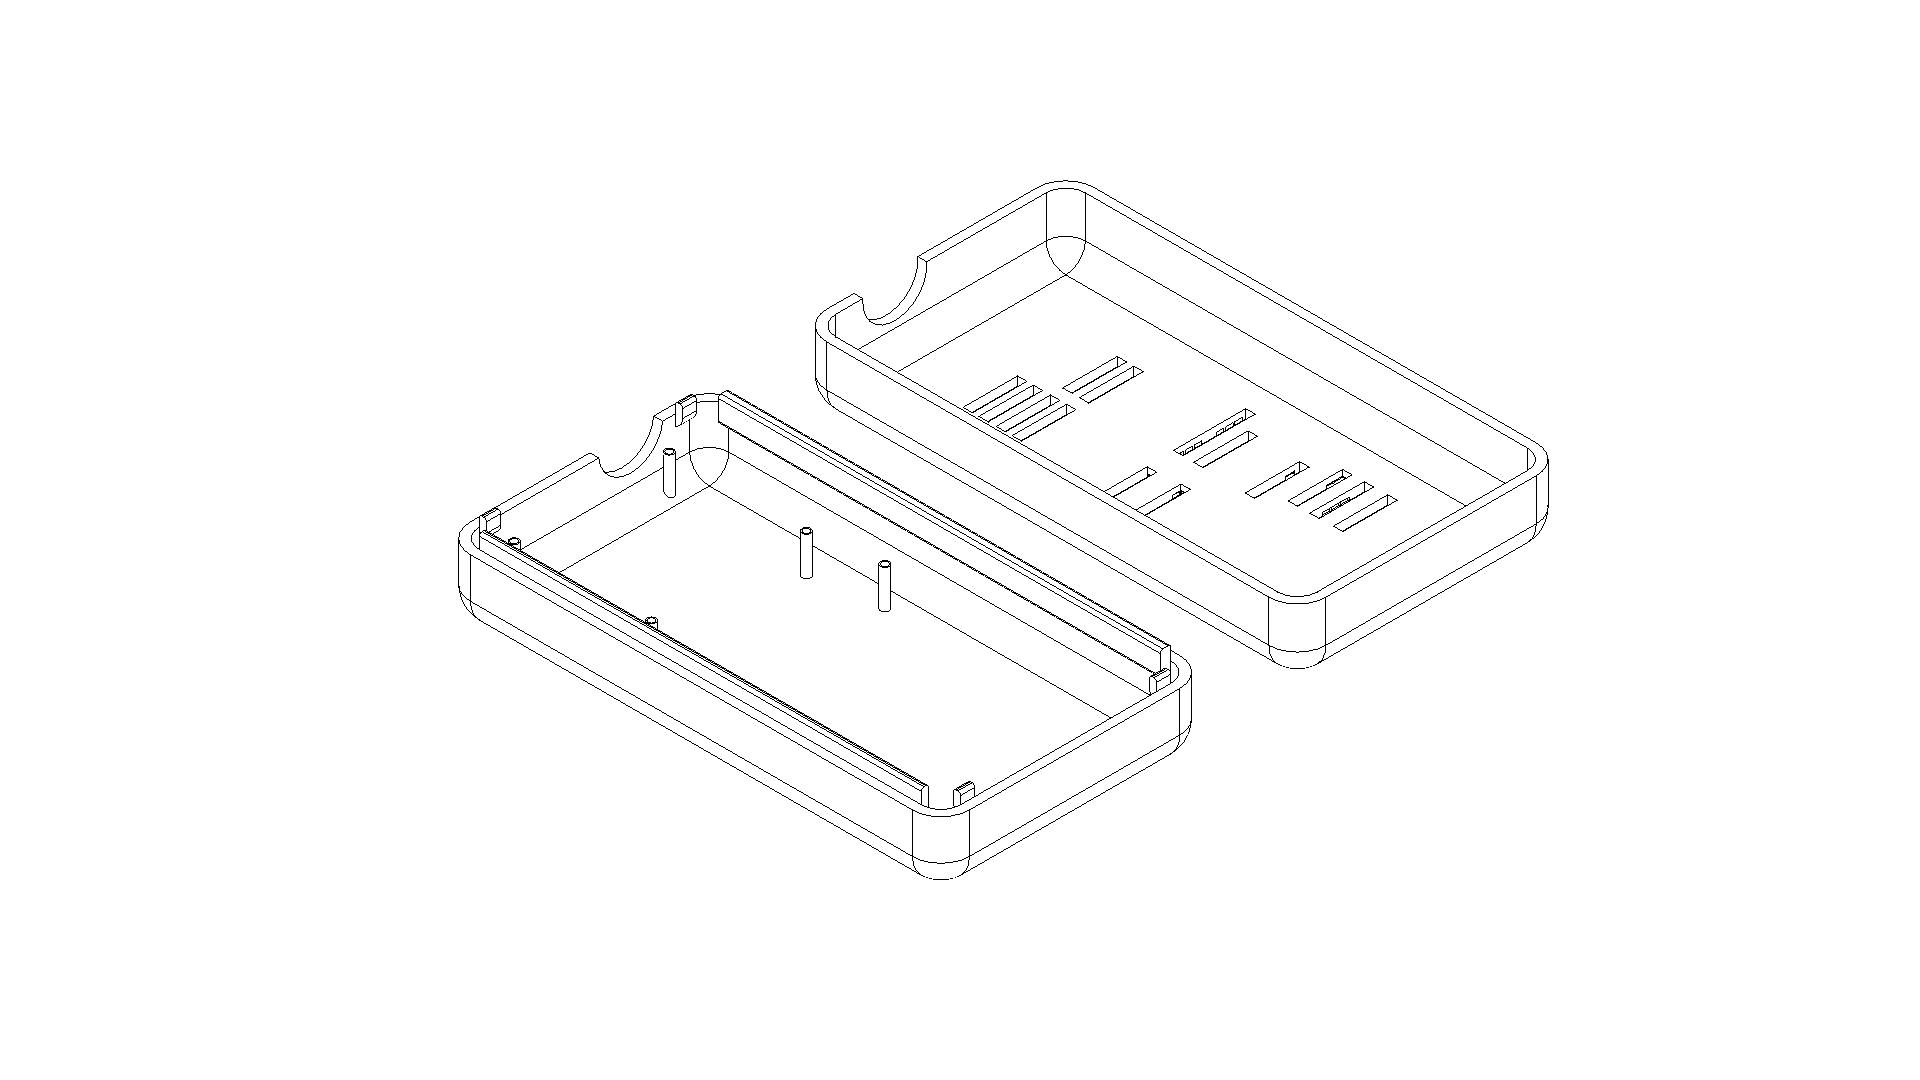
\includegraphics[width=\textwidth]{../assets/pcb/image9.jpg}
  \caption{Open Enclosure for Power Supply PCB and Peripherals PCB}
\end{figure}


\subsubsection*{STM32 Microcontroller Enclosure}
The STM32 enclosure was designed with the same principles of protection and
accessibility but tailored specifically to house the microcontroller and its
associated components. It featured openings for all essential ports, including
USB, power, and communication ports, ensuring seamless integration with other
devices and systems.


The enclosure's robust design protected the STM32 board from physical damage
and environmental factors while maintaining airflow through ventilation slots
to ensure thermal stability. Just like the power supply and peripherals
enclosure, it was created as a two-part assembly, which facilitated quick
access to the microcontroller during testing or maintenance.

\begin{figure}[H]
  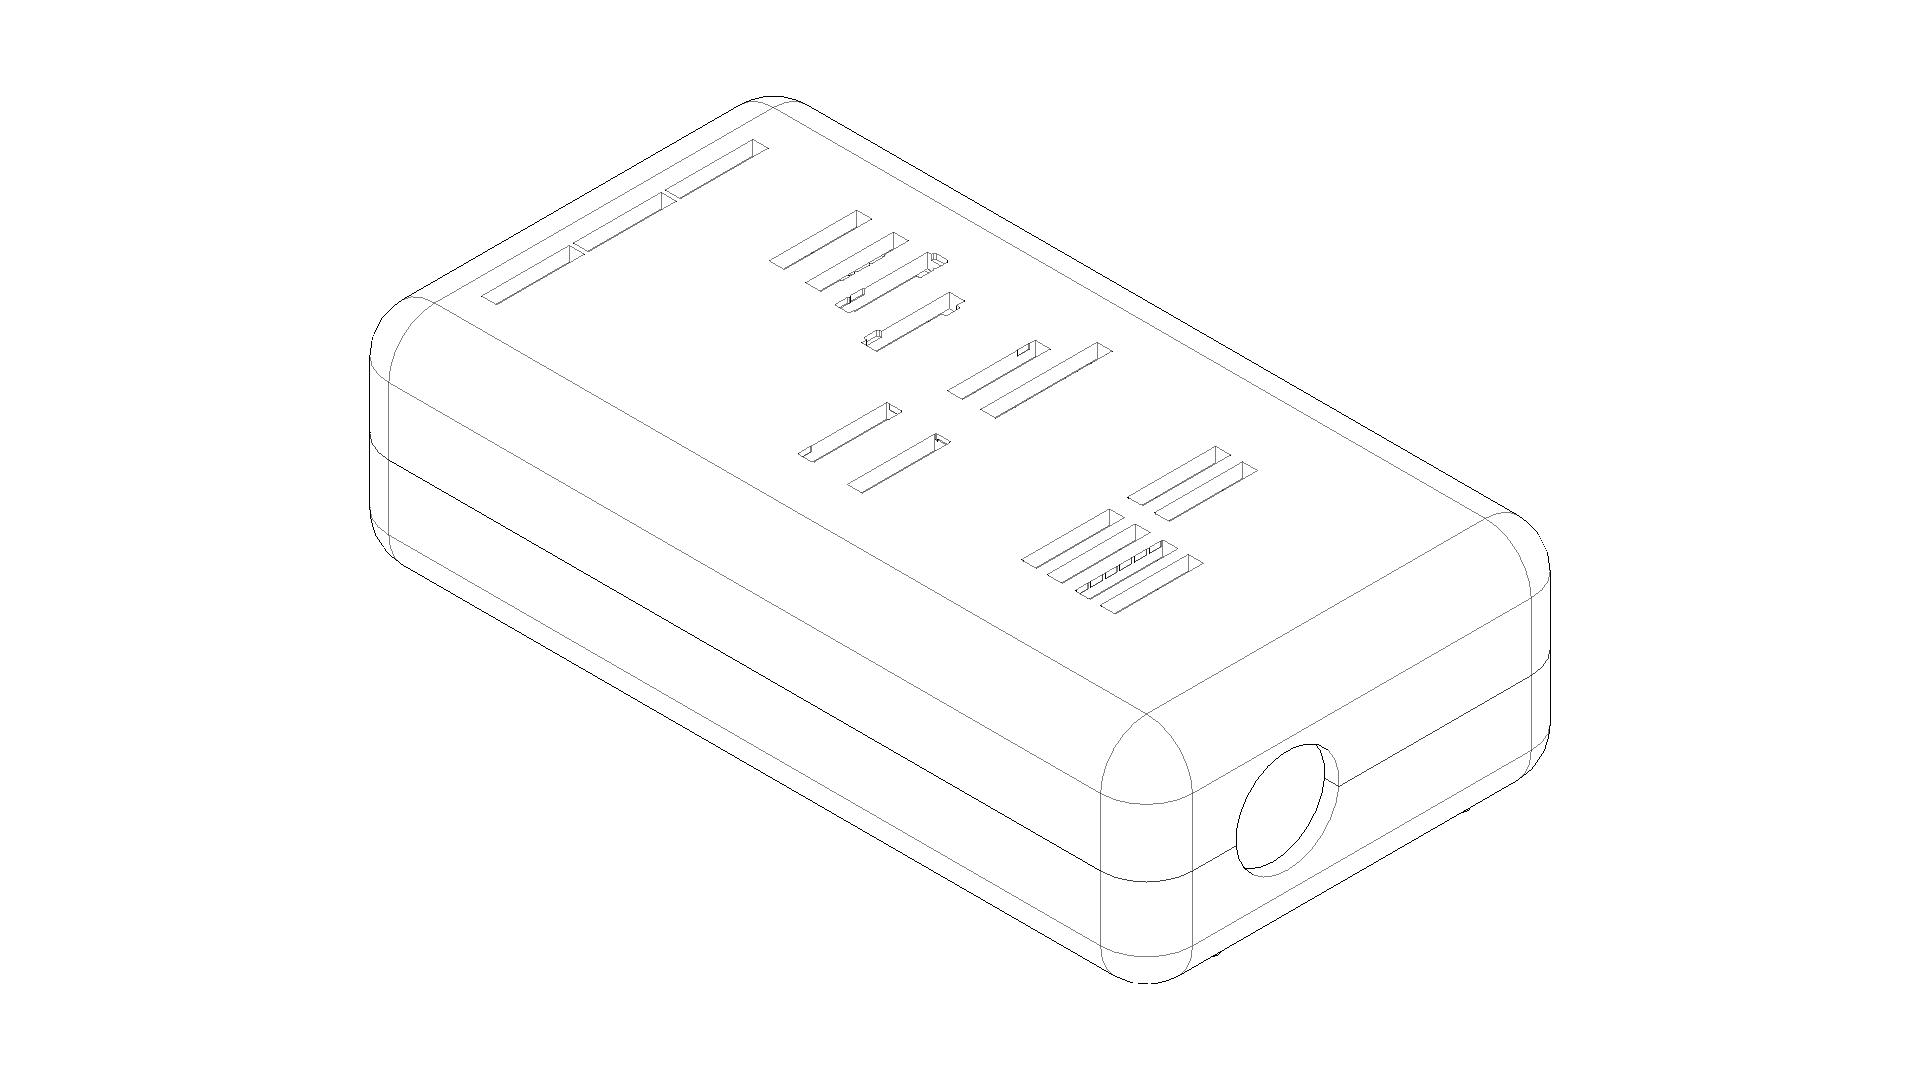
\includegraphics[width=\textwidth]{../assets/pcb/image10.jpg}
  \caption{Enclosed Enclosure for the STM32 Board}
\end{figure}

\begin{figure}[H]
  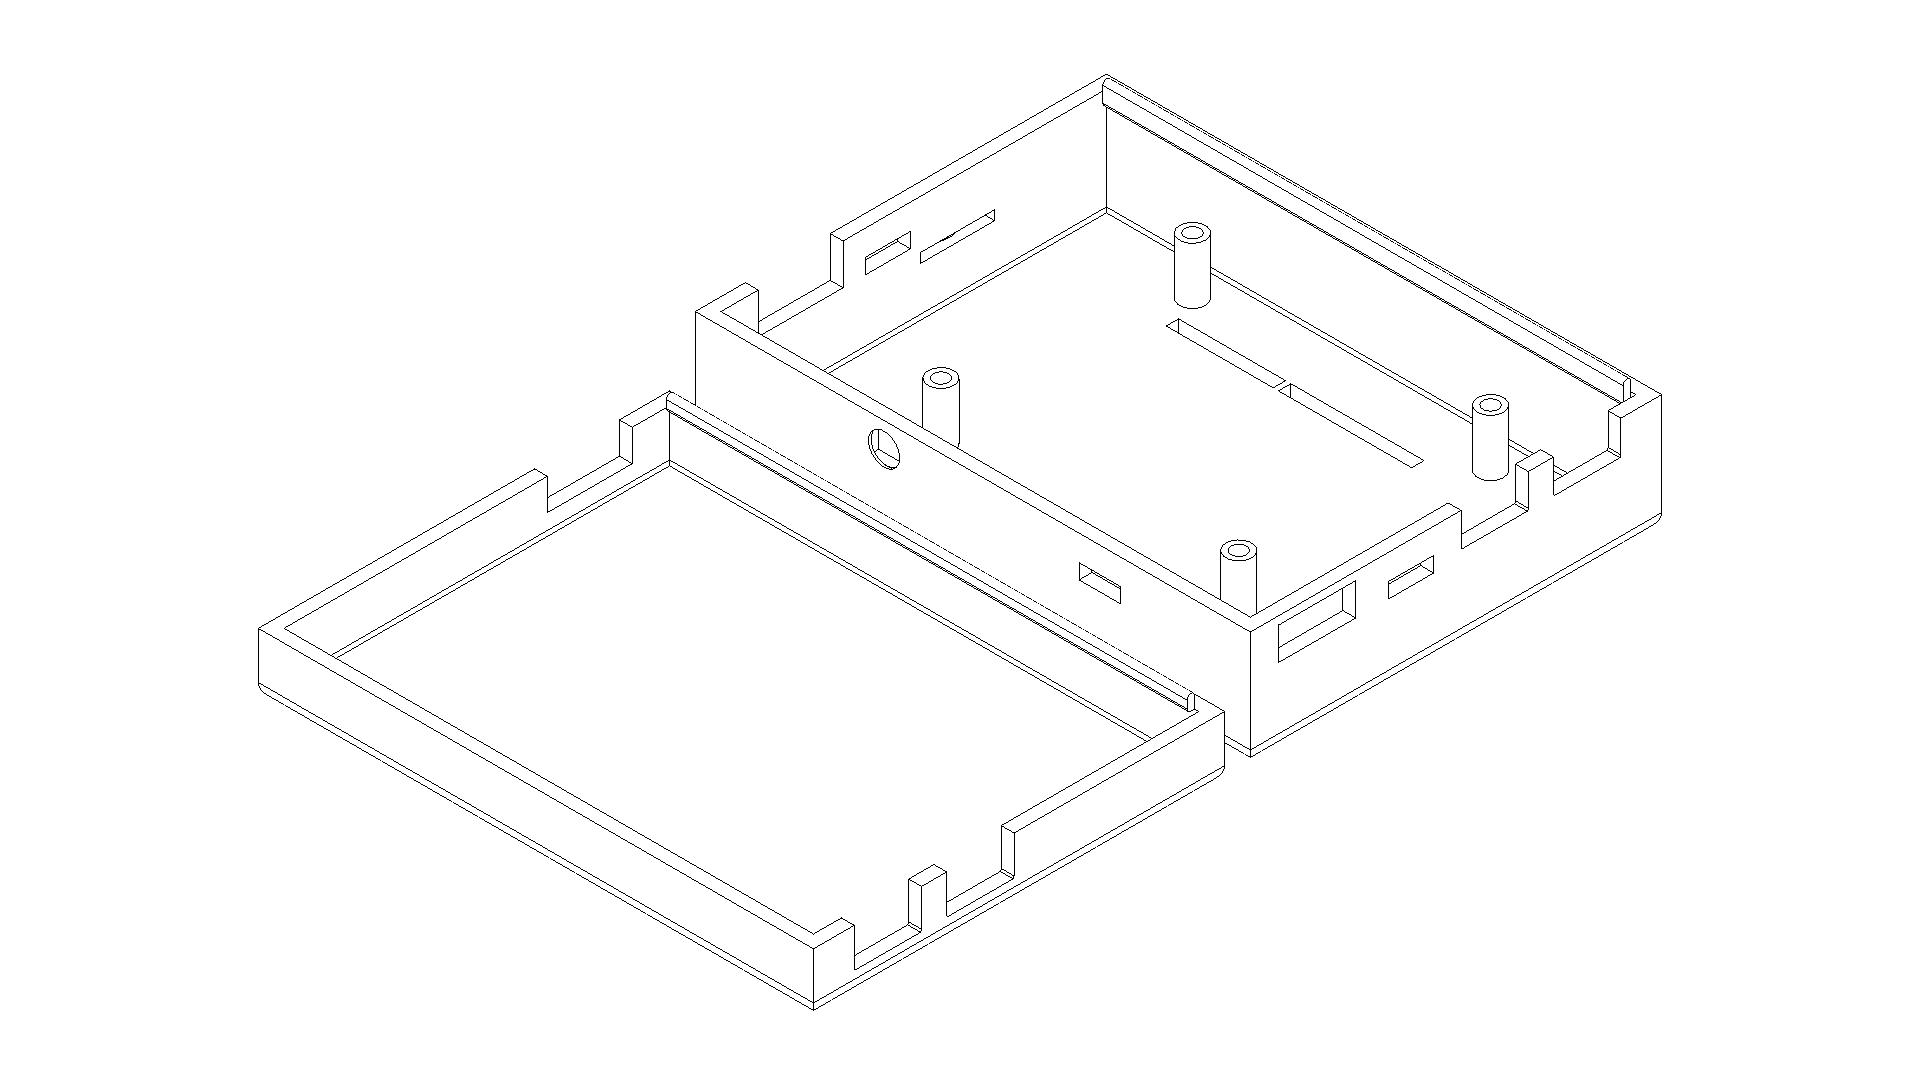
\includegraphics[width=\textwidth]{../assets/pcb/image11.jpg}
  \caption{Open Enclosure for the STM32 Board}
\end{figure}


\subsection{Arm Cortex-M4 Firmware}

\subsubsection{Brake Signal Transmitter (BST) Testing}

\subsubsection{Continuous Wear Sensor (CWS) Testing}

\subsubsection{Electronic Stability Control Module (ESCM) Testing}

\subsubsection{Pressure Sensor Testing}

\subsection{Embedded Linux with Yocto Project}

\subsubsection{Embedded Linux}
The choice to use Embedded Linux for such an application was for various reasons:
it provided access to a wide array of open-source software (OSS) and tools, it 
has a rich set of documentation accompanies by a big community of developers, and
it is likely the easiest to develop on. 

\subsubsection{The Yocto Project}
Along with using embedded Linux, a choice to use The Yocto Project was made
as it provided the best control over creating a custom Linux distribution to
deploy as an image. It handles the metadata that is necessary to make a custom
distribution. ST provides a board-support-package (BSP) layer for developers 
so that necessary hardware, kernel configurations, and device trees are configured
for propper booting.

\subsubsection{Required Software}
In the creation of a custom layer of metadata, many configurations and pieces of software was kept in mind.
\verb+wpa_supplicant+ was the first piece of software that was installed and built, as it is a wi-fi access client
and fits the standard of IEEE 802.1 for port-based network access control. Another essential piece of software
for this solution was a webserver, which this case \verb+nginx+ as it served to be small, simple, performant, and most importantly
allowed dynamic content and Web Assembly applications to be ran on the served content. Along with these, \verb+dhcp+ or 
dynamic host configuration protocol was configured for allowing the connection to any network and have an IPv4 configured.
The \verb+systemd+ init system was used for automatically starting necessary services on boot.

\subsubsection{Building Custom Software}
Software written specifically for this project such as the Web Assembly Application required specific installation
instructions in order to be deployed properly on the target image. An attempt was made to use the build system to
fetch the source of the Web Assembly application to build, but many issues and errors arose from such, and it was
determined that simply fetching the generated binary and associated files was the fastest way. From then it was simply installed
to the appropriate directory on the target device, as per the build 'recipe' by The Yocto Project.

The Custom API Rust Server was build through a provided metadata layer, \verb+meta-rust-bin+ where it contained
a Rust cross compiler that can build a generated 'recipe' by Rust's \verb+cargo+ tool by the \verb+bitbake+ crate. From
then it was simply installed to be recognized as a recognized binary on the linux filesystem as \verb+zf-server+.

The Cortex-M4 firmware were also simply installed as files, pulled from a git repository. It was installed with
an associated script to properly load the firmware to the Cortex-M4.

\begin{figure}[H]
  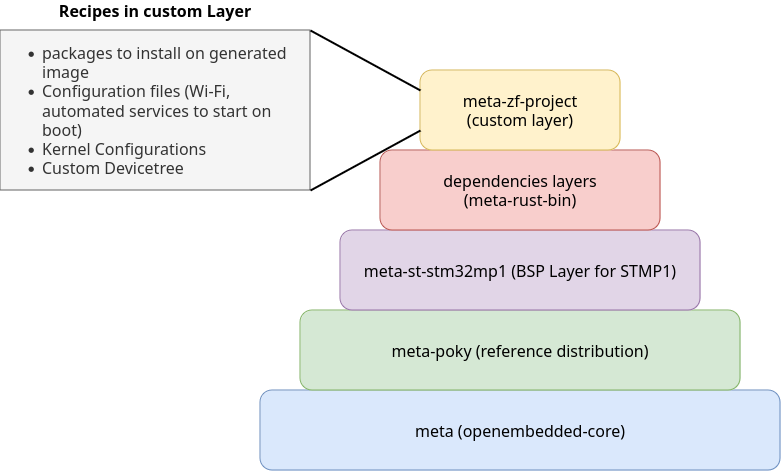
\includegraphics[width=0.75\textwidth]{../assets/layers.png}
  \caption{visualization of metadata layers under the Yocto Project}
\end{figure}


\subsection{Inter-Processor Communication with OpenAMP Project}
The STM32MP157F-DK2 contains a single system-on-chip (SoC) to house both processors (Cortex-A7 and Cortex-M4). 
Due to this locality, no traditional serial communication is allowed, therefore communication must be done through
some shared memory. 

\subsubsection{The OpenAMP (Asymmetric Multi-Processing) Project}
The OpenAMP Project is a project that seeks to standardized heterogenous architecture communication. Such
is done through a standard communication protocol of shared memory between the application processor 
and the peripheral processor. Both ends use the \verb+virtio+, which serves as a standard of communication between
virtual devices.

\subsubsection{Cortex-A7 (Linux)}
The virtual device created on the end of the Cortex-A7 is the file \verb+/dev/ttyRPMSGx+, where x
can be any number starting at 0 to however many are defined to be opened. This file serves as a bridge of
communication to the peripheral processor as writing to the file sends a message and reading from the file
recieves the message. 

\subsubsection{Cortex-M4 (Microcontroller)}
On the Cortex-M4 an additional layer of abstraction was used as it was provided by 
ST's library for development, \verb+virt_uart+ where it treated communication as if it were a UART
device. Messages would be received on the abstraction of UART and can be interpreted as a normal \verb+char*+
type in C code. 

\subsubsection{Kernel Trace Logging}
Additionally, this opened up addtional resources for the Cortex-M4 to access, namely a kernel trace log.
The firmware is now able to log information directly into the Linux filesystem through the kernel in real-time.
Because of this, when data is measured on the firmware, it is simply logged and latter is saved, to be served as 
a CSV file.

\begin{figure}[H]
  \centering
  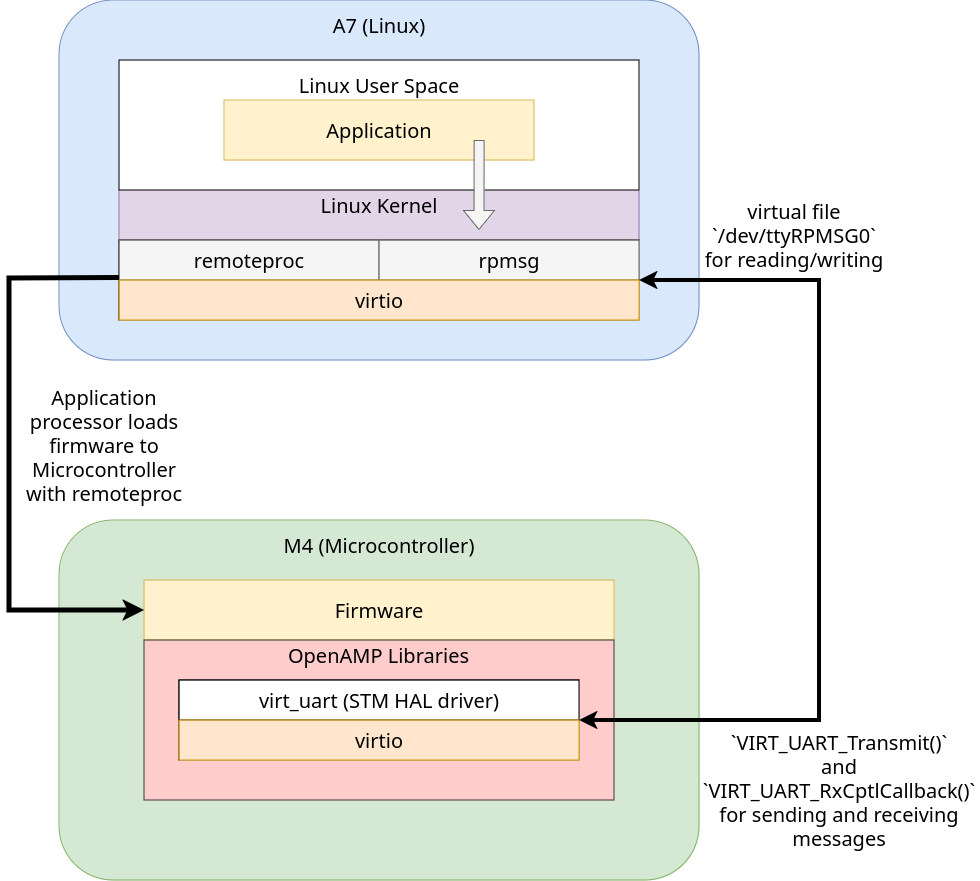
\includegraphics[width=0.75\textwidth]{../assets/ipc.drawio.png}
  \caption{Diagram of how communication on the two processors is performed}
\end{figure}

\subsection{Web Assembly Application using the Yew framework}
\subsubsection{Rust Programming Language}
Before describing the web application, the Rust Programming Language needs to be
mentioned first as it is a relatively novel language compared to most languages
used for common application. The Rust Programming language serves to be a safe alternative to
low-level languages like C while still performing near, or as well as C. It is a compiled language that
uses a LLVM backend (clang or anything not GNU). It is commonly being looked at as an alternative more
and more as it becomes more used. The use of it in this project aims to push this potential to
one day serve as a replacement to the C programming language.

\subsubsection{Web Assembly}
Web Assembly is another feature in the web application that is far more novel. It exists to solve the slow
runtime of Javascript by using a binary format executable where a script (Javascript) would have normally been used.
A common language to be compiled into Web Assembly is Rust as Rust does not have a grabage collector, which greatly
increases the compatability of being used as a Web Assembly binary. In this case, the Yew framework is used to develop
the entire Web Assembly application.

\subsection{User Interface}
The user interface (UI) is kept simple to remove ambiguity and mantain focus on the functionality. 
The user is greeted with a button to select a device with a button, and the UI updates depending on which the
user has clicked on. Specifically for the BST, an option to use the with the string potentiometer is provided, as this
affects how the firmware tests the DUT. Once the user clicks the "Start test" button, an HTTP request is sent
to the web server to begin the test. The web appliation polls the server for the test completion. Once the web application receives 
the response that the test has been completed, the UI is updated to reflect either a pass or fail, with a new button
appearing to download the associated CSV file.

\begin{figure}[H]
  \centering
  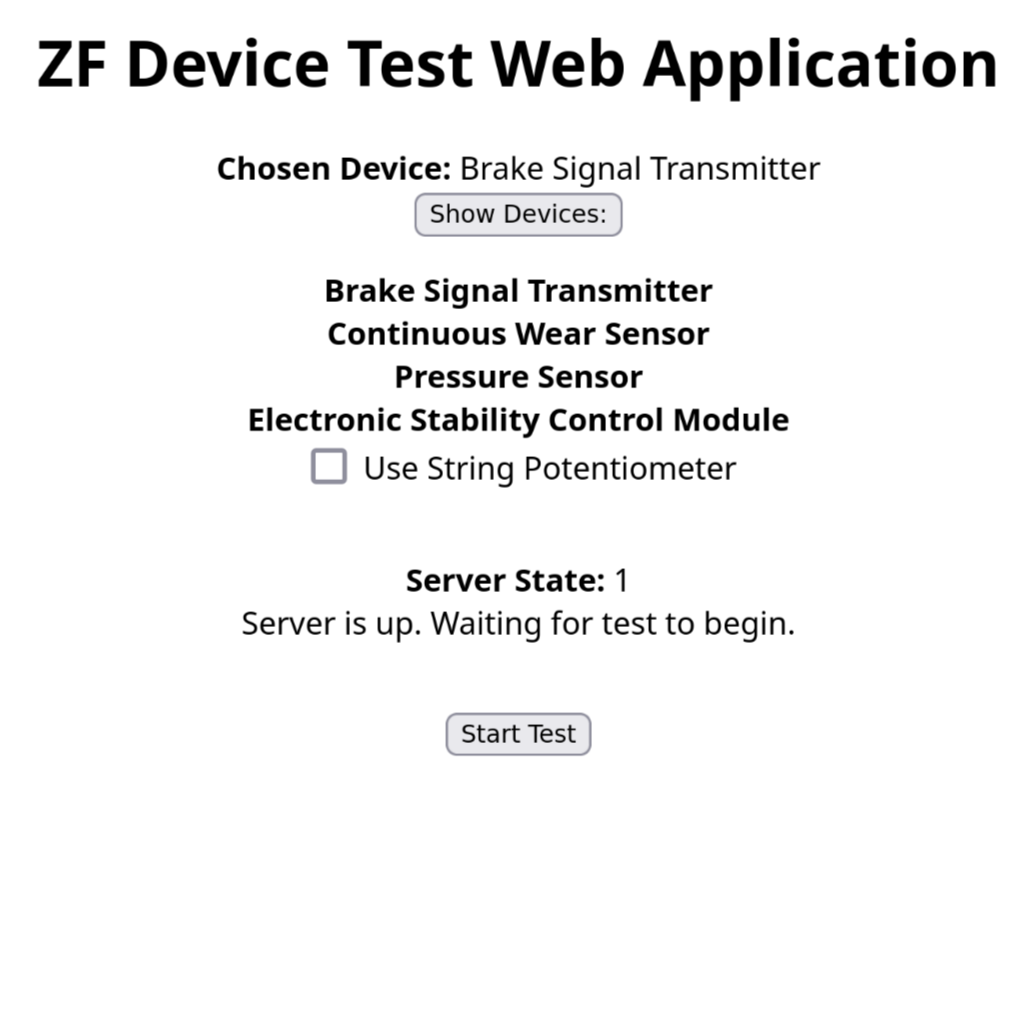
\includegraphics[width=0.5\textwidth]{../assets/webapp.png}
  \caption{Image of web application with drop down menu for different devices}
\end{figure}

\subsection{Custom API Web Server in Rust}
\subsubsection{Designing Custom API}
The Web server was designed not follow any standard API as it served to be unecessary. The server will only ever interact with
the specific associated web application and will not need to follow any standards for response codes. For this reason, all responses
sent by the web server are in pure bytes and unserialized.

\subsubsection{Loading Firmware}
The server uses the \verb+warp+ Rust crate to ensure the correct request is being handled. 
Once the information of a device is recieved for a test to start, the server
determines which device test firmware to load into the Cortex-M4. Once loaded,
the server checks \verb+/dev/ttyRPMSG0+ to see if it exists, as this confirms whether or not 
the firmware successfuly opens the bridge for Inter-processor communication. 

\subsubsection{Saving CSV Data}
Once testing, the server polls the firmware every 500ms for completion. Once
it receives a message it is complete, the firmware saves the kernel trace log under
\verb+/sys/kernel/debug/remoteproc/remoteproc0/trace+ as \verb+<device name>-data.csv+ and
is available for download as a path request on the web application.

\begin{figure}[H]
  \centering
  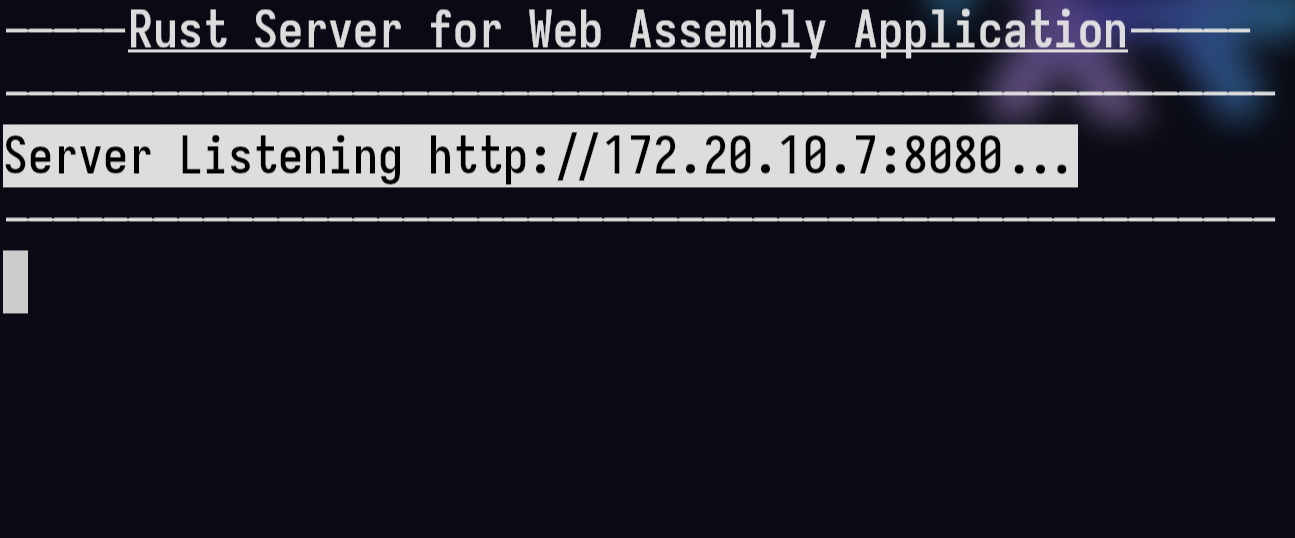
\includegraphics[width=0.5\textwidth]{../assets/server1.png}
  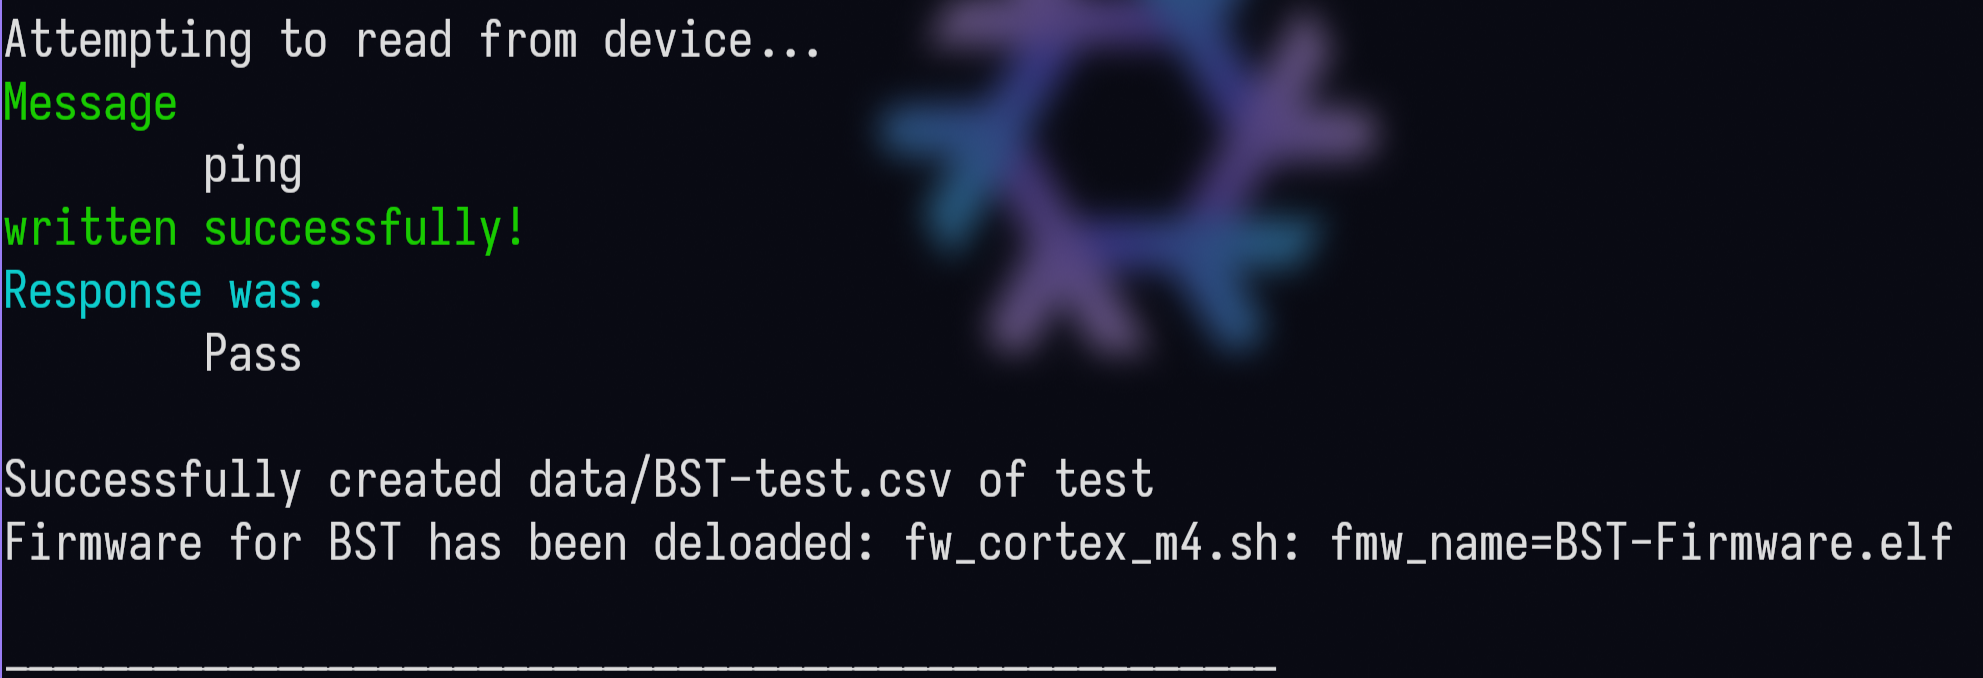
\includegraphics[width=0.75\textwidth]{../assets/server2.png}
  \caption{Console logging of server}
\end{figure}

\subsection{Comprehensive Software Interaction Diagram}

\begin{figure}[H]
  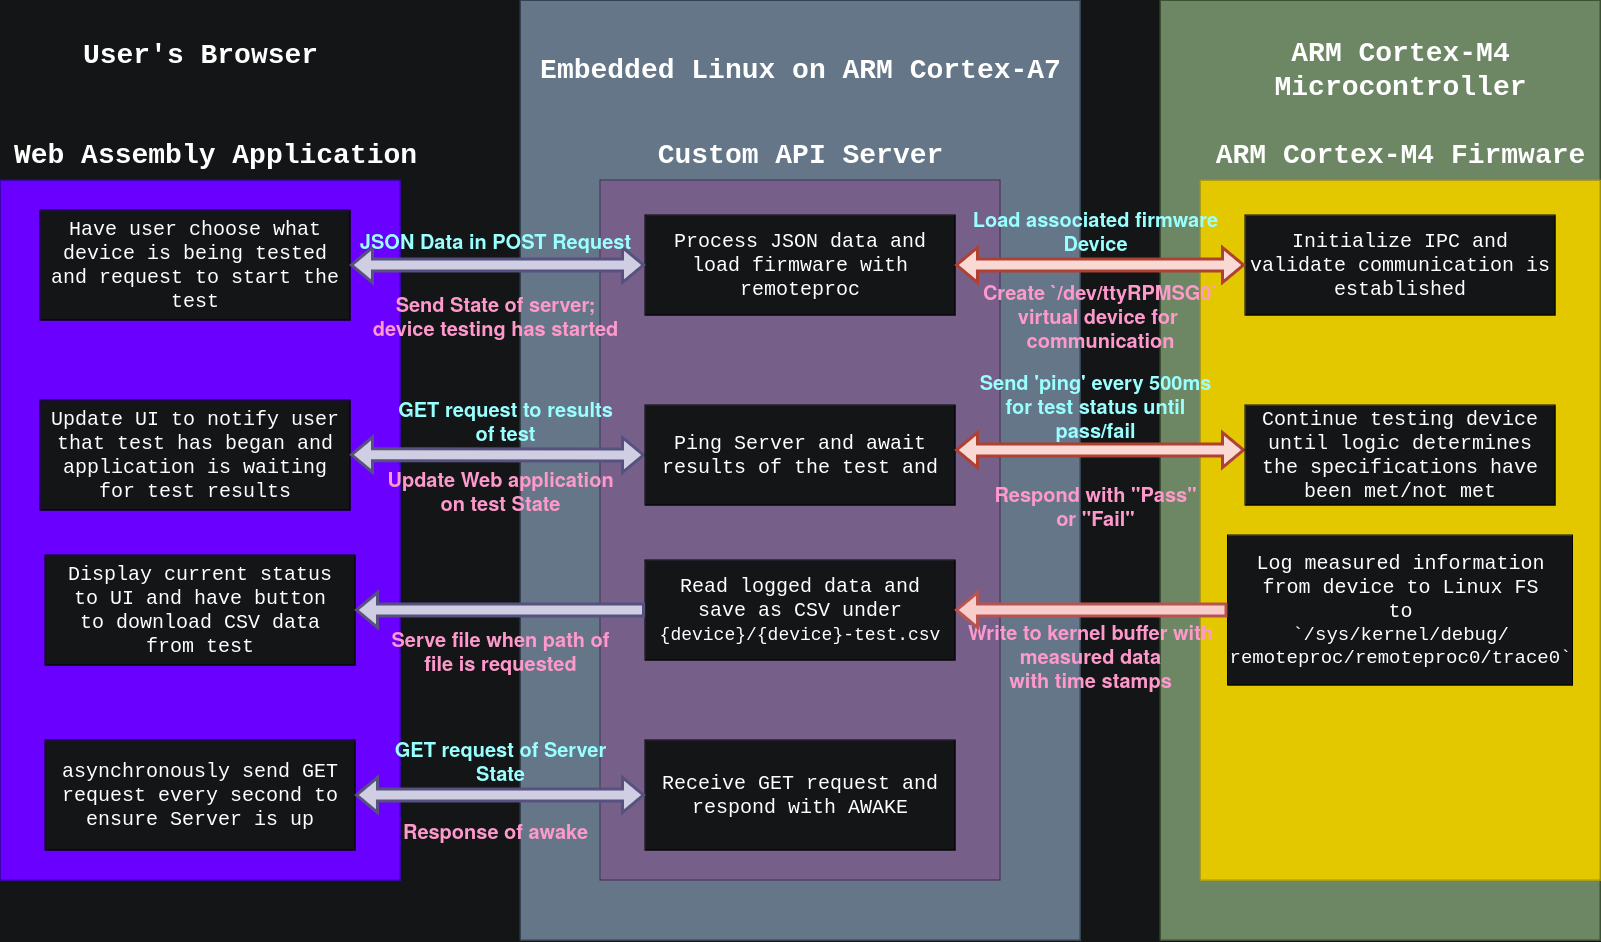
\includegraphics[width=\textwidth]{../assets/software_stack.drawio.png}
  \caption{Comprehensive diagram of different platforms interacting from web-browser to Cortex-M4}
\end{figure}

%----------------------------------------------------------------------------------------
%	Design Considerations 
%----------------------------------------------------------------------------------------
\subsection{Design Considerations}
When designing the Multi-Signal Automotive Testing Device, several factors were
taken into consideration to ensure the project aligns with broader societal,
environmental, and economic goals.

\subsubsection{Public Health}
This device ensures accurate testing of automotive components, contributing
indirectly to public health by improving vehicle safety. For example, properly
functioning brake signal transmitters and stability control systems can reduce
accidents, keeping roads safer for everyone.


\subsubsection{Safety and Welfare}
Safety was prioritized in the design process. The enclosures were crafted to
protect the electronics from physical damage, and the use of standoffs and
secure mounts minimizes risks of electrical short circuits. Additionally, the
circuit design incorporated diodes to prevent reverse voltage damage, ensuring
operational reliability.


\subsubsection{Global Impact}
The design supports the development of safer automotive systems globally. Since
cars are used worldwide, this project contributes to the larger goal of
enhancing vehicle reliability and reducing accidents, which has a ripple effect
on public safety and environmental sustainability.


\subsubsection{Cultural Impact}
Automotive systems impact people differently based on their cultural
priorities. In cultures where vehicle ownership represents progress and
economic stability, this device indirectly supports technological advancement
and trust in automotive technology.


\subsubsection{Social Impact}
Automotive systems impact people differently based on their cultural
priorities. In cultures where vehicle ownership represents progress and
economic stability, this device indirectly supports technological advancement
and trust in automotive technology.

\subsubsection{Environmental/Sustainability}
The device was designed with energy efficiency in mind. For instance, voltage
regulators and capacitors were used to ensure efficient power consumption.
Furthermore, the focus on durability and modularity reduces electronic waste
since individual components can be replaced rather than discarding the whole
device.


\subsubsection{Economic}
Economically, this device helps lower testing costs for automotive systems by
providing a reliable and reusable solution. The use of custom PCBs and locally
designed enclosures ensured cost efficiency while maintaining functionality.

%----------------------------------------------------------------------------------------
%	Design Impacts
%----------------------------------------------------------------------------------------
\subsection{Design Impacts}
The project had several direct and indirect impacts on a variety of domains,
from the global stage to individual communities.

\subsubsection{Global}
On a global scale, this project aligns with the push for smarter, safer, and
more reliable automotive systems. It enhances the tools available for testing
automotive components, which is critical in the development of advanced
driver-assistance systems (ADAS) and autonomous vehicles.

\subsubsection{Economic}
The device minimizes testing costs for automotive manufacturers, especially for
smaller companies that may lack access to expensive testing equipment. Its
modular design allows cost-effective upgrades, ensuring long-term usability.


\subsubsection{Environmental}
The environmental impact was reduced by selecting components that support
energy efficiency and reducing waste through a modular design. Additionally, by
enabling more reliable testing of components like brake and wear sensors, this
project indirectly reduces environmental hazards caused by vehicle failures.


\subsubsection{Societal}
The societal impact of this project lies in its ability to enhance safety
standards. Reliable testing leads to safer vehicles, which means fewer
accidents, lower healthcare costs, and better public trust in transportation
infrastructure.



%----------------------------------------------------------------------------------------
%	Performance and Testing Analysis
%----------------------------------------------------------------------------------------
\subsection{Performance and Testing Analysis}


%----------------------------------------------------------------------------------------
%	Conclusion
%----------------------------------------------------------------------------------------
\pagebreak
\section{Conclusion}

The Claims Investigation Committee Multi-Testing Input Device project
successfully delivered a comprehensive testing solution for ZF Group's
automotive safety components. The system effectively automates validation
testing across multiple devices including the Brake Signal Transmitter,
Continuous Wear Sensor, and pressure sensors, addressing the key challenges
faced by the Claims Investigation Center.

The implemented solution combines robust hardware design with modern software
architecture. Custom PCBs manage power and signal routing, while the dual-core
STM32MP157F-DK2 platform handles both real-time signal processing and test
management. The WebAssembly frontend and Rust backend provide an intuitive user
interface, with OpenAMP facilitating seamless inter-processor communication.

Test results demonstrate the system's capability to validate components against
manufacturer specifications through automated data collection and analysis. The
platform's modular design supports multiple device types and allows for future
expansion. Notably, the system achieves significant improvements in testing
efficiency compared to manual methods, while maintaining the rigorous standards
required for automotive safety component validation.

Despite challenges in system clock configuration and PCB creation, the project
fulfilled its primary objectives of streamlining the validation process and
enhancing the CIC's testing capabilities. Future work will focus on completing
CAN implementation for ESCM testing and further refinements to the web
application interface.

\section{Recomendations}
For developing on this project further, potentially as another Senior Design Project,
several recomentations can be made for improving current features, fully implementing 
features not finished, or extending functionality. 

Improving the apperance of the web application is a very simple feature to begin
improving. To extend on the web application, porting it from using the Yew 
Web Assembly framework to simple Web Assembly modules with valls to Javascript 
for Document-Object-Model manipulations would enhance the portability of this portion
greatly for easier development.

A feature to finish implementation of is propper usage of the onboard CAN module 
by implementing pin-multiplexing on the Yocto device tree.

For a complete, comprehensive improvement, a completely custom PCB can be designed 
with all the different components of the STM32MP157F-DK2 properly connected
and laid out. 




\end{document}
